\documentclass[article]{jlreq}
\usepackage[dvipdfmx]{graphicx}
\usepackage{here}
\usepackage{amsmath}
\usepackage{latexsym}
\usepackage{multirow}
\usepackage{textcomp}
\usepackage{url}
\usepackage{array}    % 列の設定
\usepackage{caption}
\usepackage{booktabs}
\usepackage[utf8]{inputenc}
\usepackage{subcaption}
\newcommand{\ita}{\textit}
\newcommand{\ko}{\rm{k$\Omega$}}
\newcommand{\om}{\rm$\Omega$}
\newcommand{\nf}{\rm{nF}}
\title{}
\date{}
\begin{document}\maketitle



\section{実験1}
以下に実験1で用いた回路を示す。

\begin{figure}[H]
    \centering

    \begin{minipage}{0.48\linewidth}
        \centering
        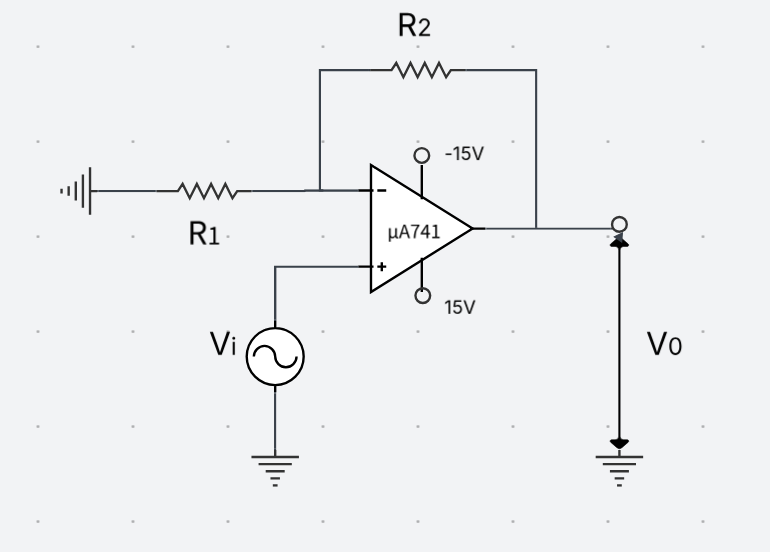
\includegraphics[width=\linewidth]{hihuku.png}
        \caption{非反転増幅回路}
    \end{minipage}
    \hfill
    \begin{minipage}{0.48\linewidth}
        \centering
        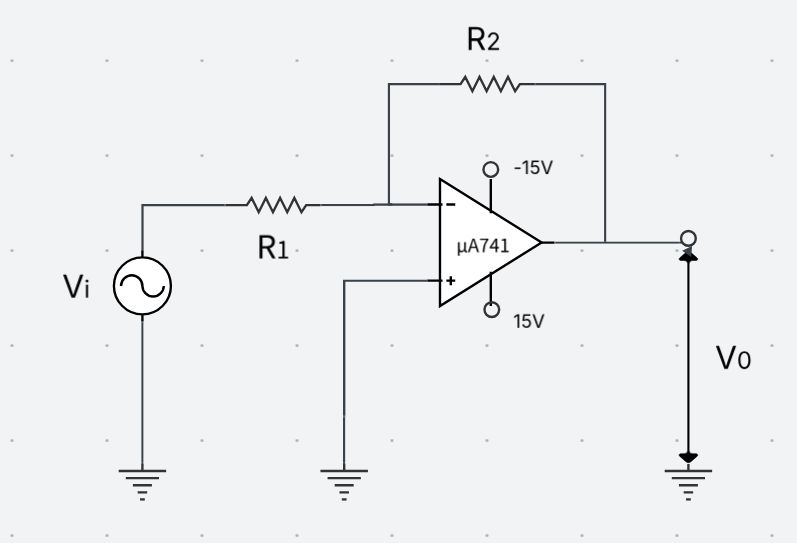
\includegraphics[width=\linewidth]{huku.png}
        \caption{反転増幅回路}
    \end{minipage}

\end{figure}

\subsection{非反転増幅回路の特性}
\subsubsection{実験内容}
\begin{enumerate}
\item 図1の回路において,$R_1 = 1\,\text{k}\Omega $に対し,$R_2 = 1\,\text{k}, 10\,\text{k}, 100\,\text{k}\Omega$ と設定し,$V_i$ として,振幅
$V_{AMPL} = 1\,\text{V}$,周波数$ f = 1\,\text{kHz} $の正弦波を入力したときの出力波形を観察した。
以下にLTspiceにより作成した回路図を示す。
\begin{figure}[H]
    \centering
    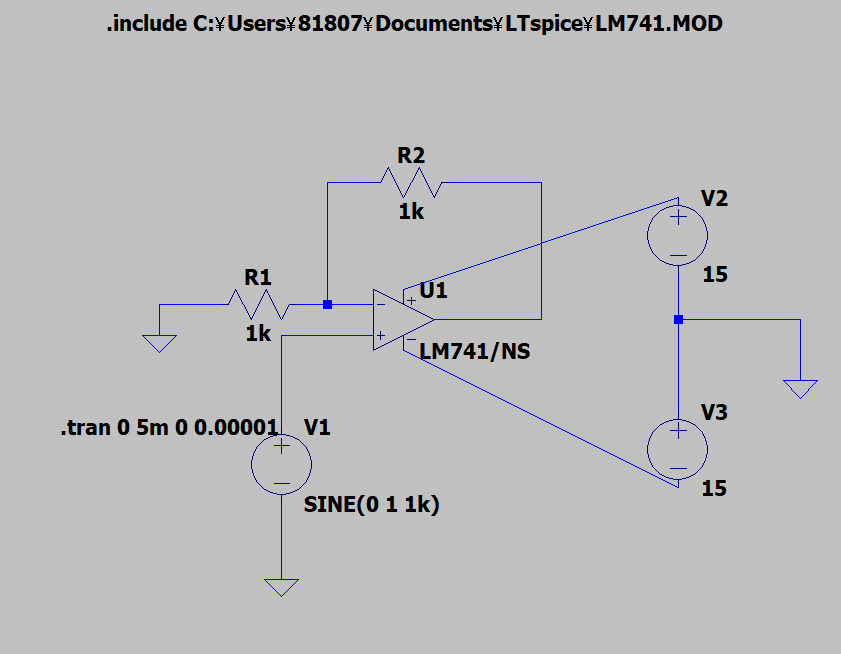
\includegraphics[scale=0.35]{kairozu5-11.png}
    \caption{$R_2 = 1\,\text{k}\Omega$}
\end{figure}
\begin{figure}[H]
    \centering
    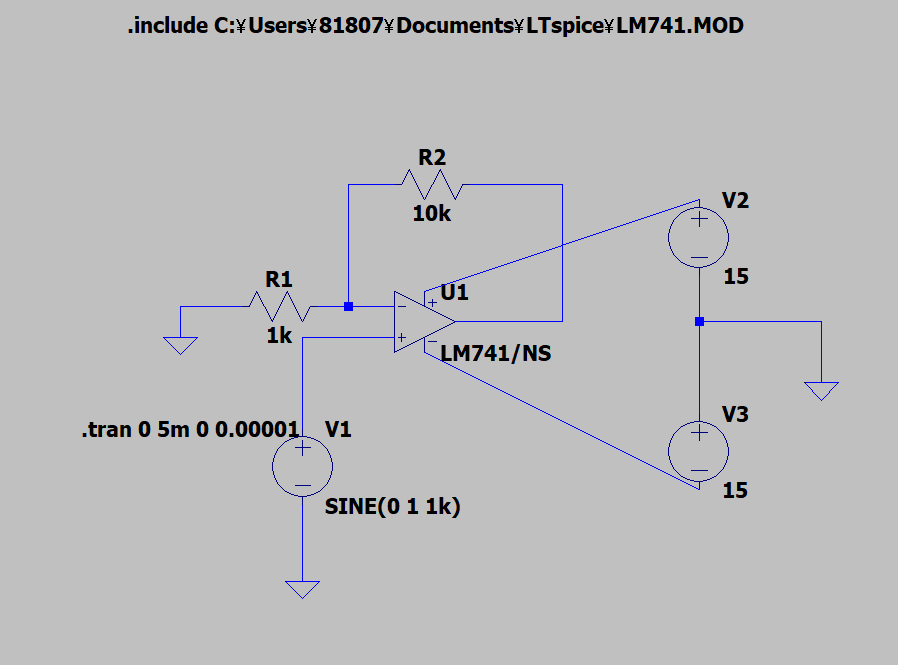
\includegraphics[scale=0.35]{kairozu5-12.png}
    \caption{$R_2 = 10\,\text{k}\Omega$}
\end{figure}
\begin{figure}[H]
    \centering
    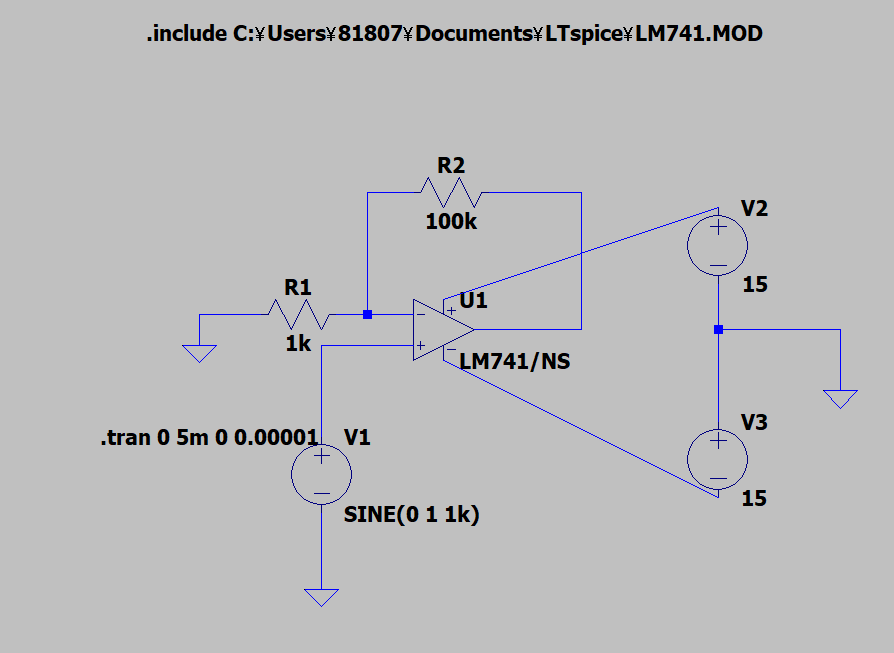
\includegraphics[scale=0.35]{kairozu5-13.png}
    \caption{$R_2 = 100\,\text{k}\Omega$}
\end{figure}

\item $R_1 = 1\,\text{k}\Omega $ に対し,$R_2 = 1\,\text{k}, 10\,\text{k}, 100\,\text{k}\Omega$と設定したときの周波数特性 (振幅特性と位相特性) を
観察した。
以下にLTspiceにより作成した回路図を示す。
\begin{figure}[H]
    \centering
    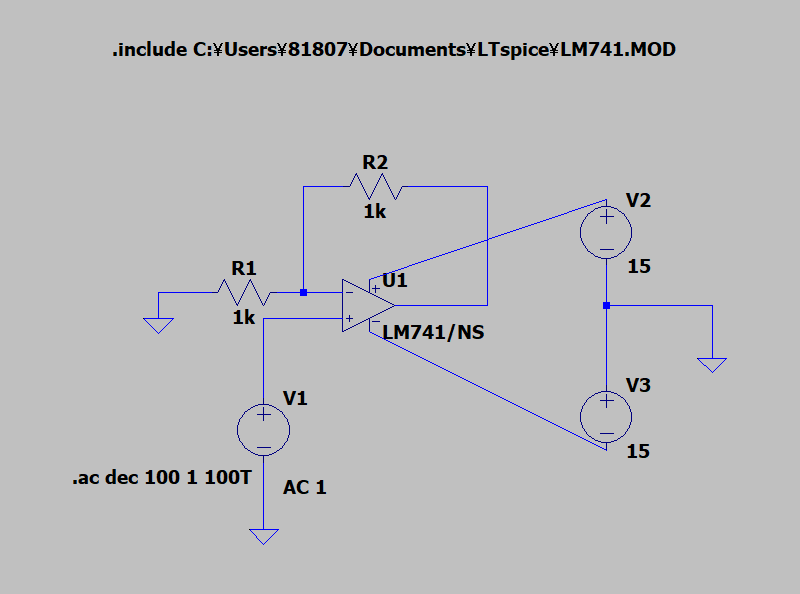
\includegraphics[scale=0.35]{kairozu5-21.png}
    \caption{$R_2 = 1\,\text{k}\Omega$}
\end{figure}
\begin{figure}[H]
    \centering
    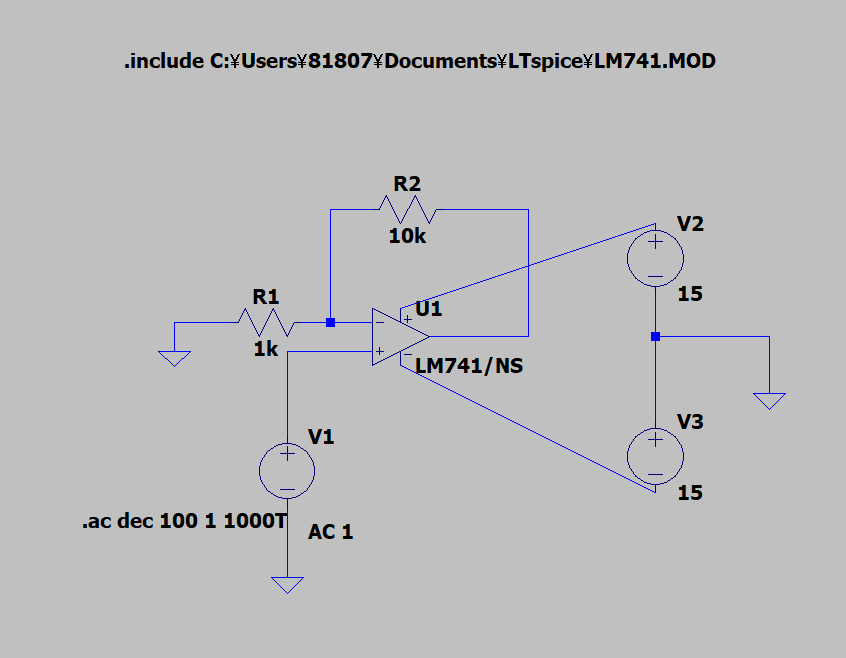
\includegraphics[scale=0.35]{kairozu5-22.png}
    \caption{$R_2 = 10\,\text{k}\Omega$}
\end{figure}
\begin{figure}[H]
    \centering
    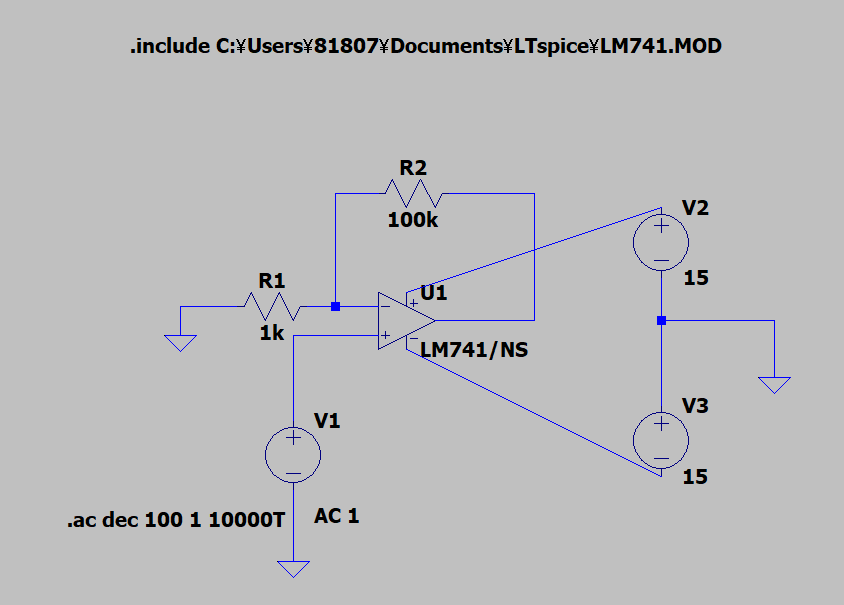
\includegraphics[scale=0.35]{kairozu5-23.png}
    \caption{$R_2 = 100\,\text{k}\Omega$}
\end{figure}
\end{enumerate}
\subsubsection{結果}
以下に各$R_2$に対する解析結果示す。
\begin{figure}[H]
    \centering
    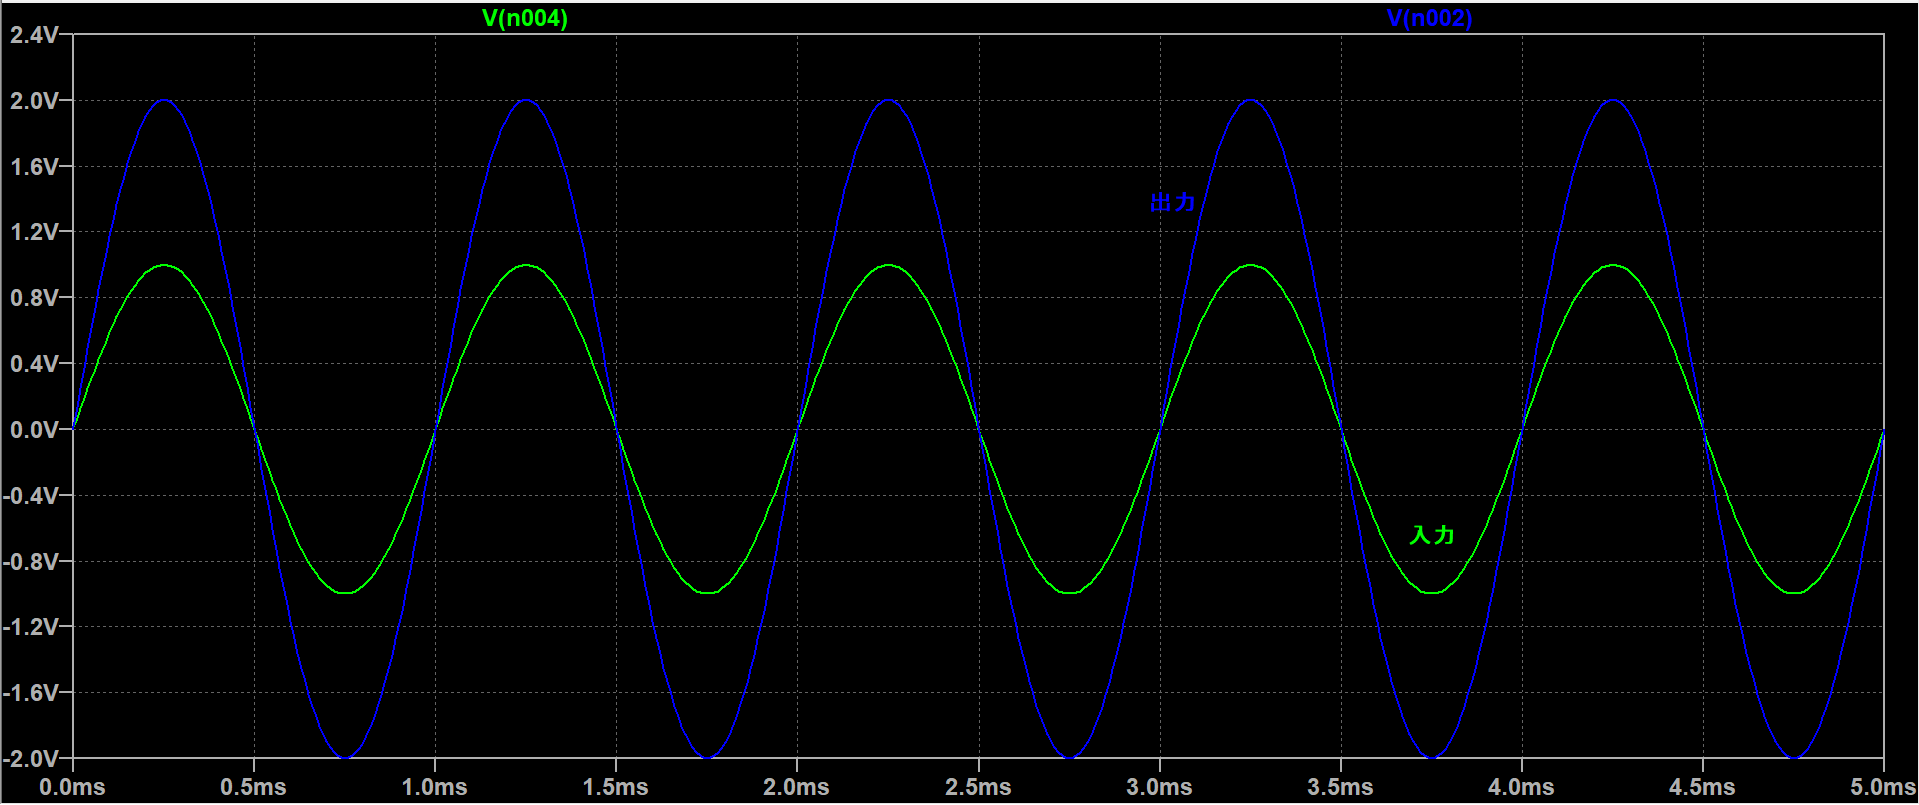
\includegraphics[scale=0.25]{sim5-11.png}
    \caption{$R_2 = 1\,\text{k}\Omega$}
\end{figure}
\begin{figure}[H]
    \centering
    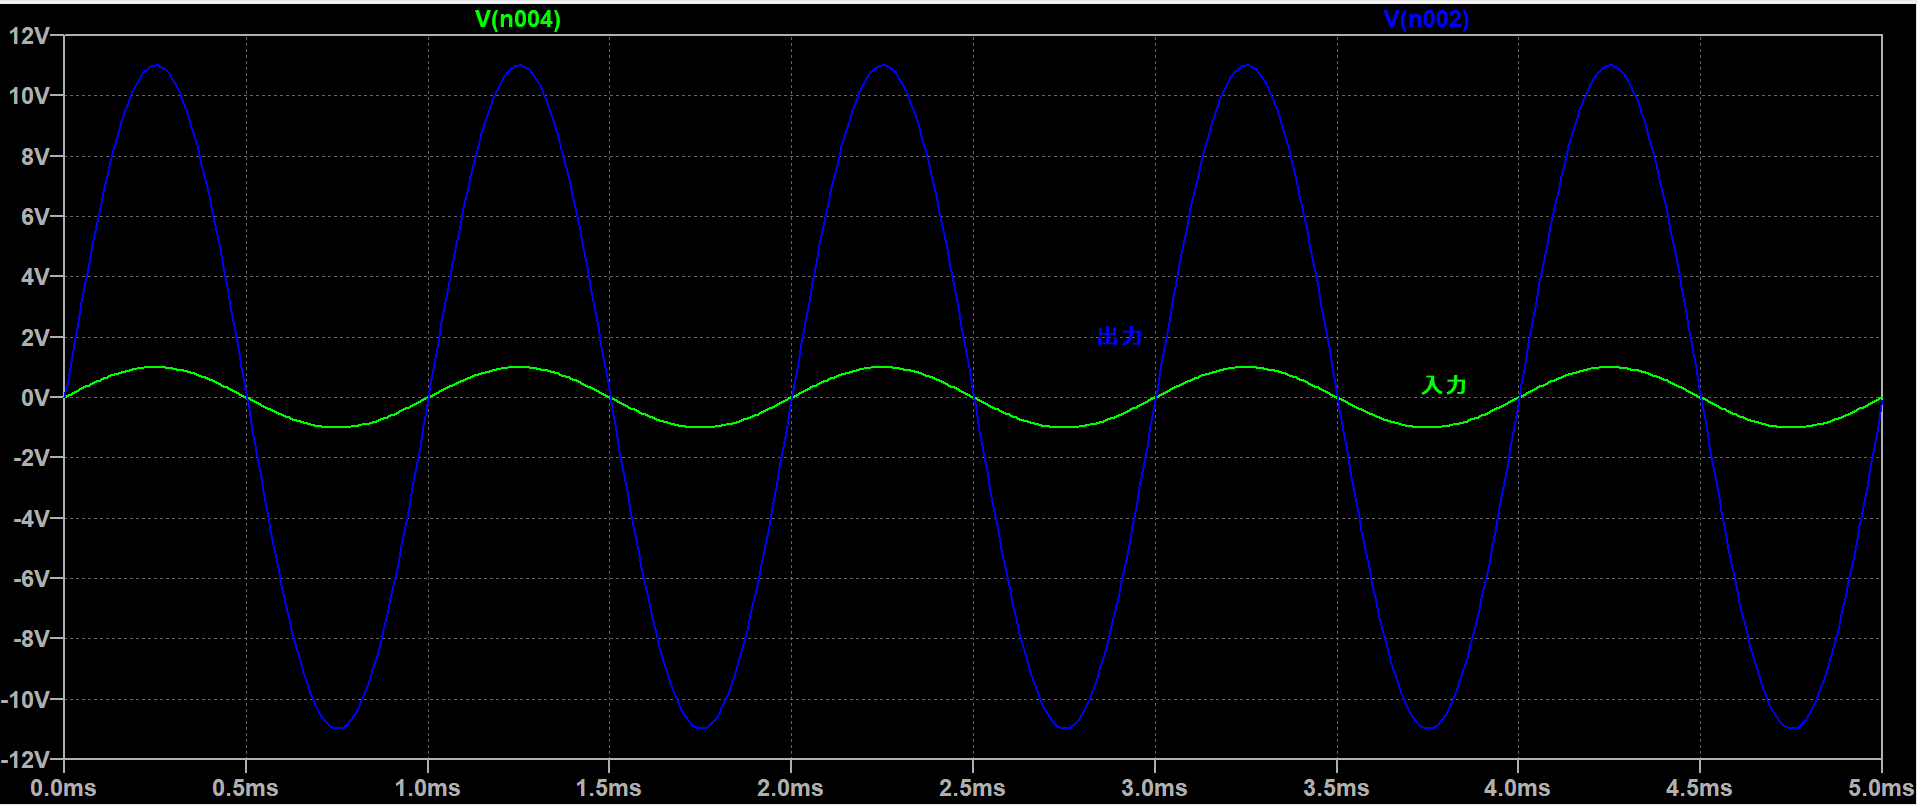
\includegraphics[scale=0.25]{sim5-12.png}
    \caption{$R_2 = 10\,\text{k}\Omega$}
\end{figure}
\begin{figure}[H]
    \centering
    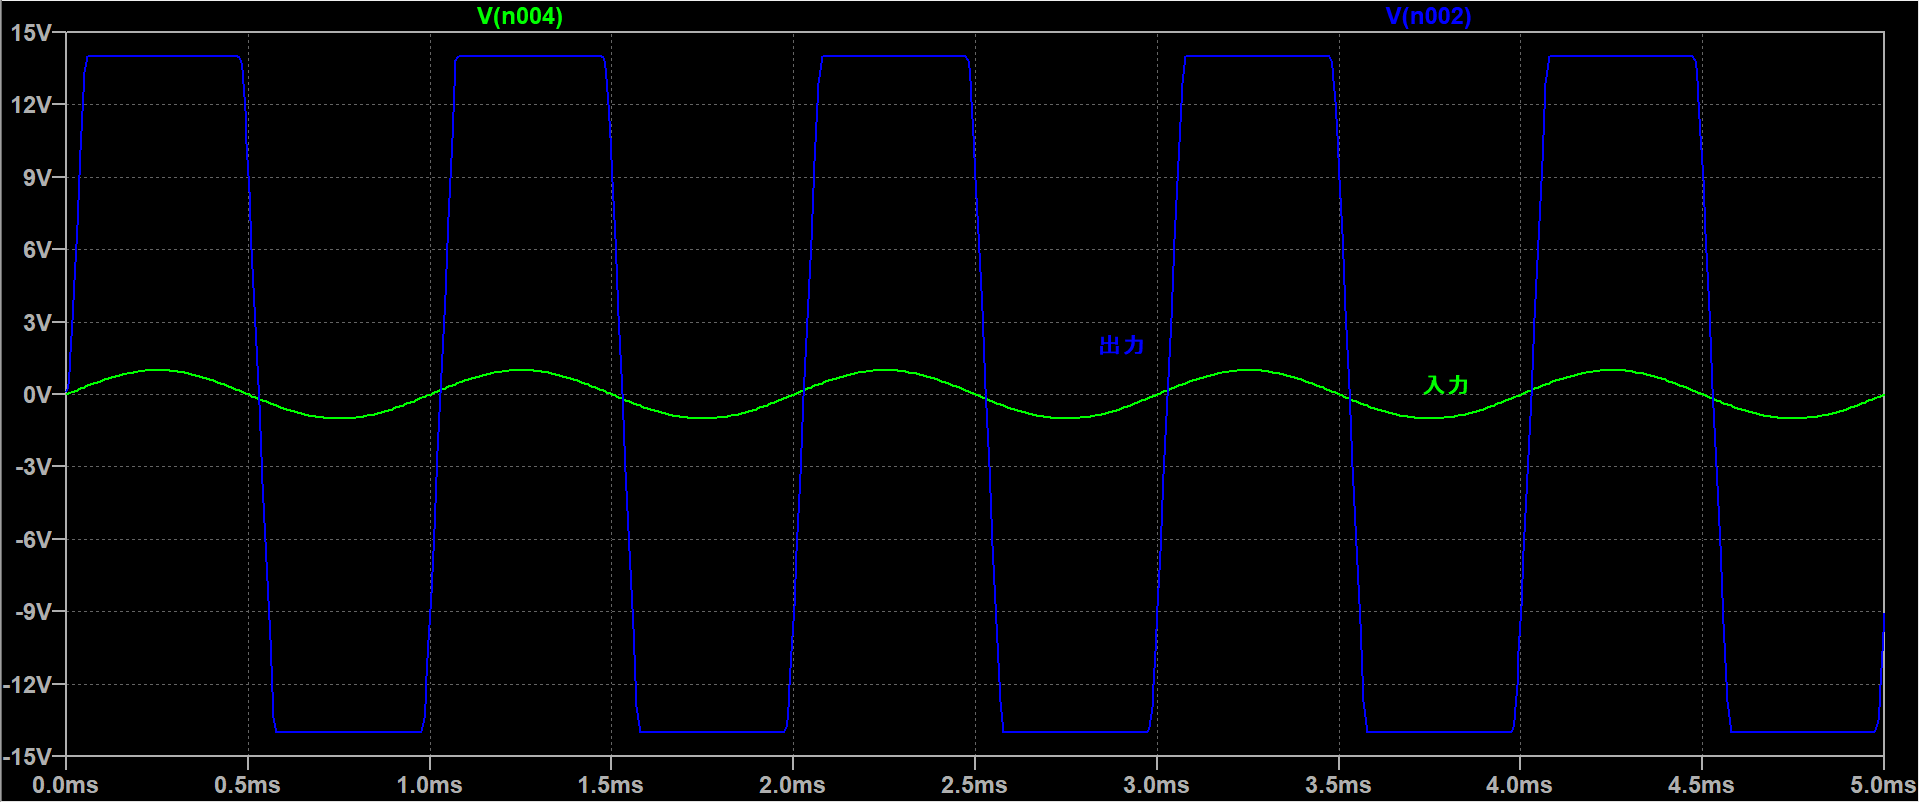
\includegraphics[scale=0.25]{sim5-13.png}
    \caption{$R_2 = 100\,\text{k}\Omega$}
\end{figure}

\begin{figure}[H]
    \centering
    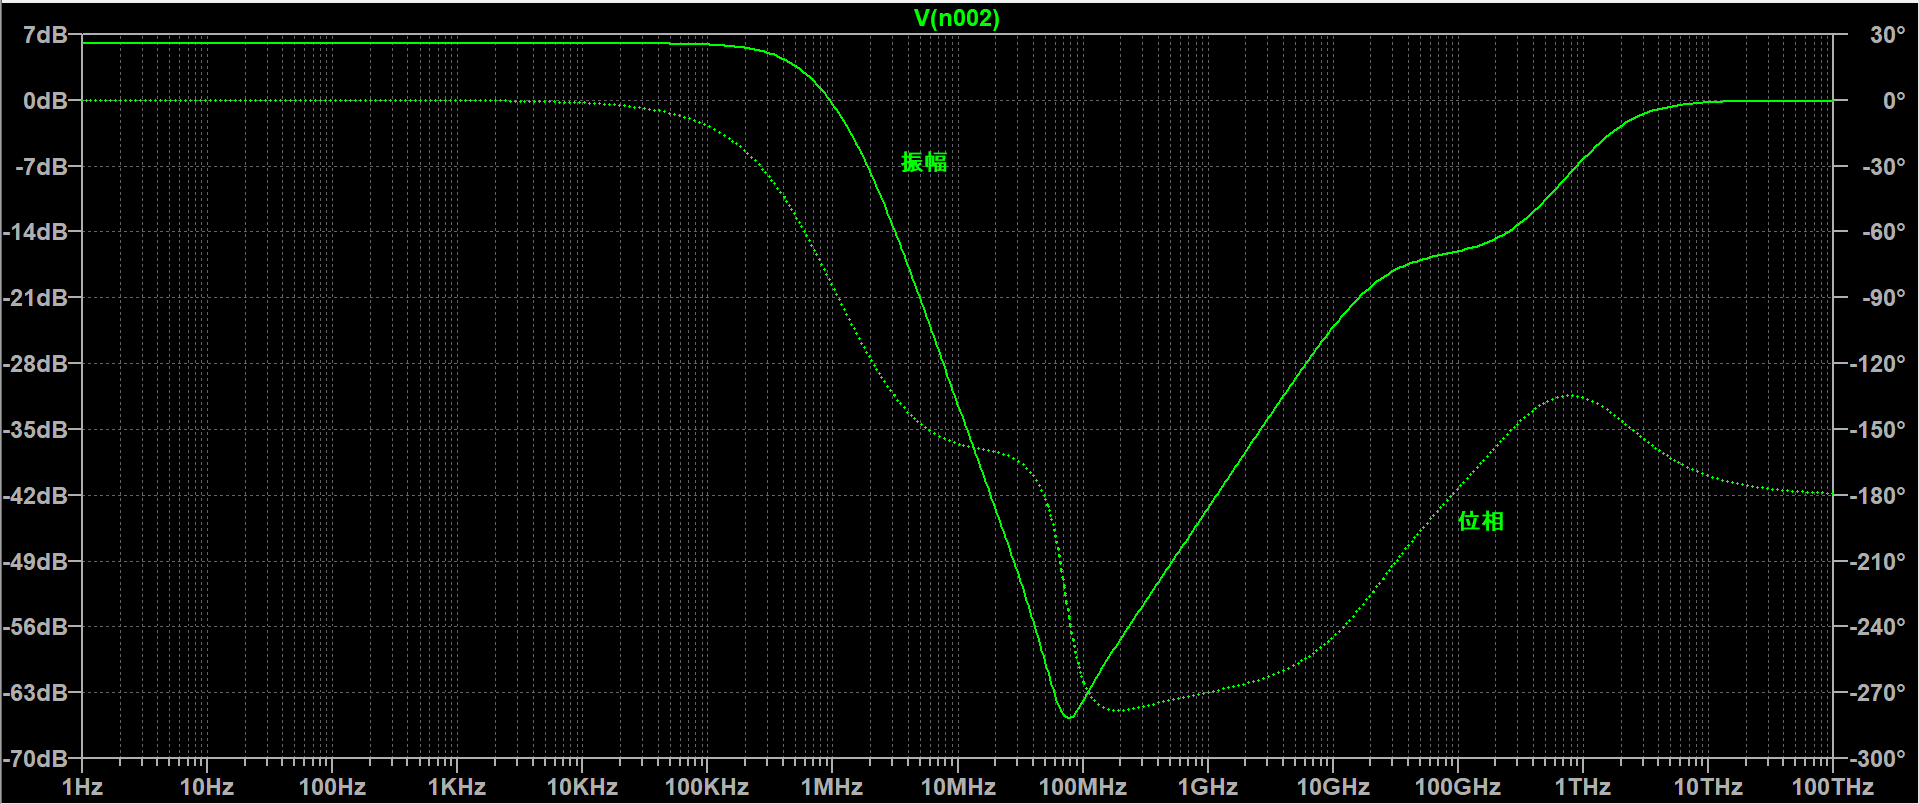
\includegraphics[scale=0.25]{sim5-21.png}
    \caption{$R_2 = 1\,\text{k}\Omega$}
\end{figure}
\begin{figure}[H]
    \centering
    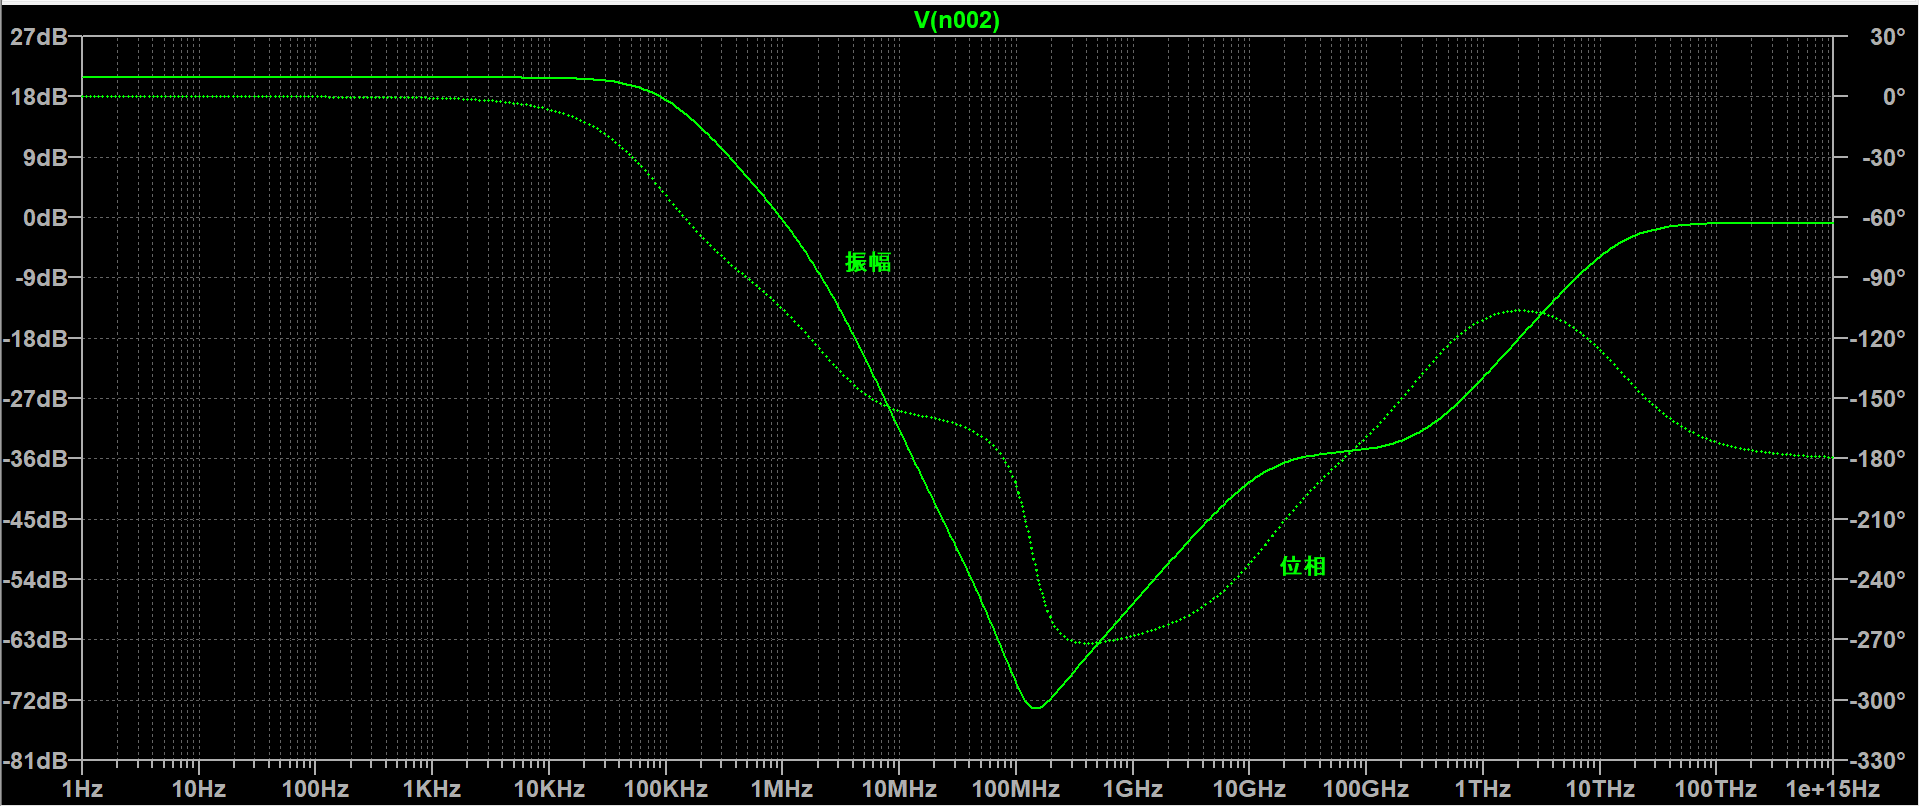
\includegraphics[scale=0.25]{sim5-22.png}
    \caption{$R_2 = 10\,\text{k}\Omega$}
\end{figure}
\begin{figure}[H]
    \centering
    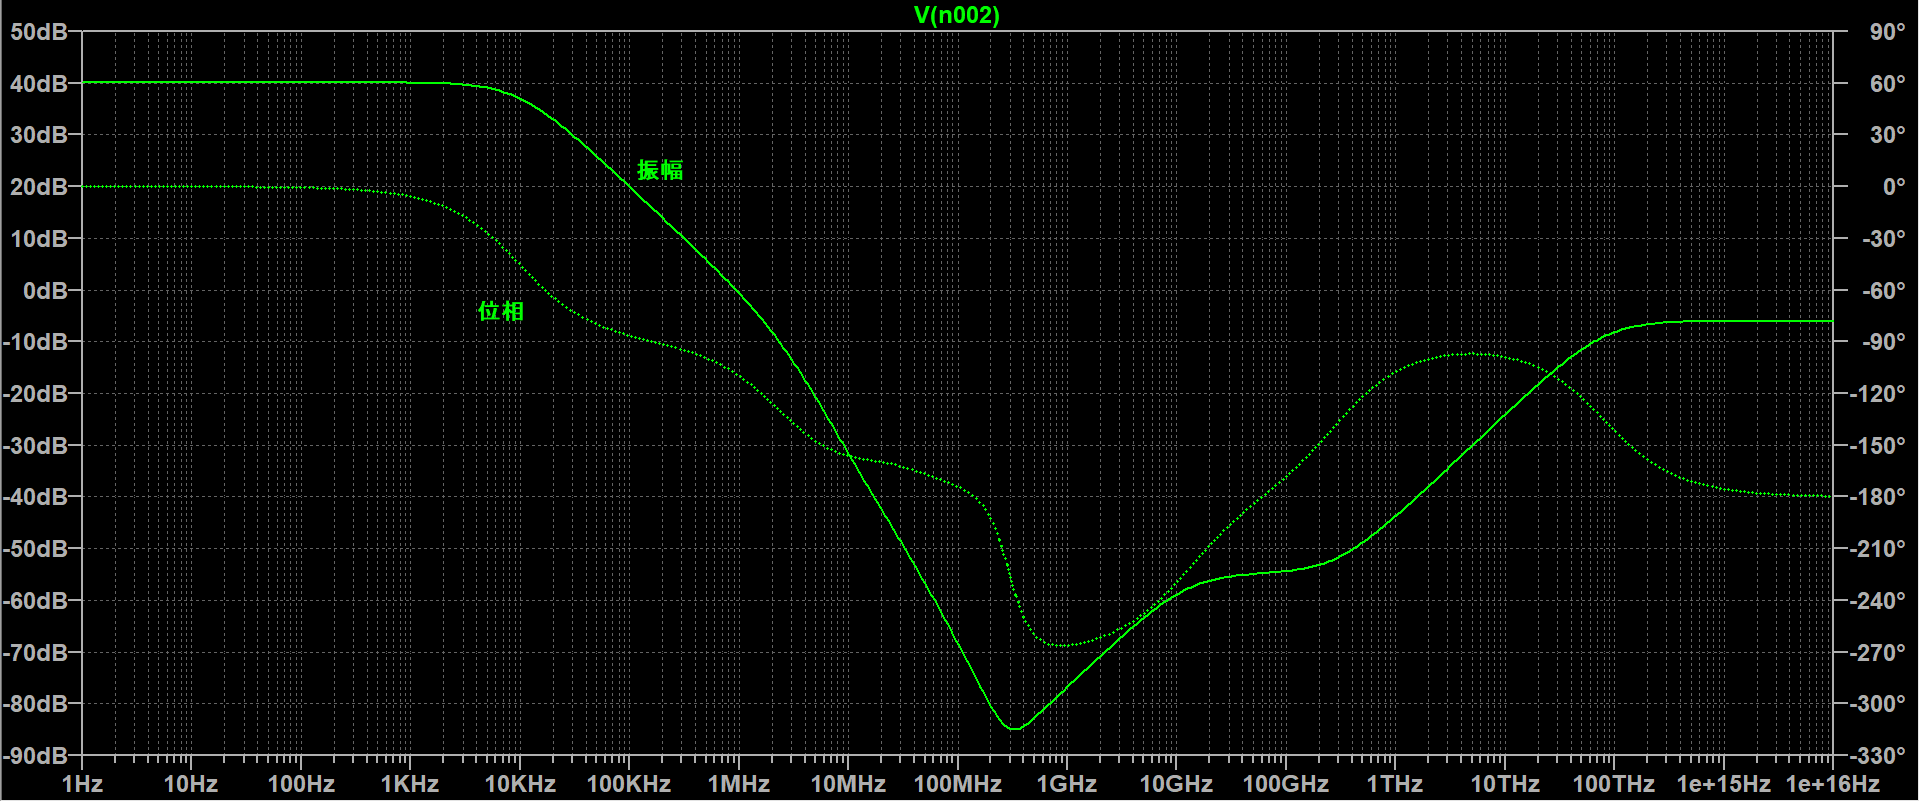
\includegraphics[scale=0.25]{sim5-23.png}
    \caption{$R_2 = 100\,\text{k}\Omega$}
\end{figure}

\subsubsection{考察}
\paragraph{考察1}\mbox{}\\
非反転増幅回路では、
$R_2$
の値を大きくすると低周波領域での利得も大きくなった。

非反転増幅回路の増幅率は

\[
A_v = 1+\frac{R_2}{R_1}
\]

で与えられるため、
$R_1=1\,\mathrm{k\Omega}$
とした今回の条件では、
$R_2$
を大きくするほど理論増幅率も大きくなる。

実際の周波数特性においても、
低周波領域ではそれぞれ約
$6\,\mathrm{dB}$、
$21\,\mathrm{dB}$、
$40\,\mathrm{dB}$
程度となっており、
理論値とほぼ一致した。

一方、
周波数を高くすると利得は低下した。
これは、
実際のオペアンプでは高周波になるほど
理想的な増幅動作ができなくなるためである。

また、
$R_2$
を大きくした回路ほど、
利得が低下し始める周波数が低くなった。
したがって、
高い増幅率を得るほど、
使用できる周波数範囲は狭くなることが確認できた。

さらに、
より高い周波数領域では、
利得が再び増加する様子が確認できた。
このことから，
高周波領域では低周波領域とは異なる動作をしており，
理想的な非反転増幅回路とは異なる特性が現れていることが確認できた。

位相特性については、
低周波領域では入力と出力は同相であり、
位相差は
$0^\circ$
であった。
しかし、
周波数が高くなるにつれて位相遅れが大きくなった。

また、
利得が再び増加する周波数領域では、
位相も大きく変化しており、
回路の動作が低周波領域とは異なることが確認できた。\\

\paragraph{考察2}\mbox{}\\
考察1で示したように、
非反転増幅回路では
$R_1 \gg R_2$
とすると増幅度はほぼ
1
となる。
したがって、
この回路は入力電圧をほぼそのまま出力する回路となる。

また、
非反転増幅回路では入力信号をオペアンプの非反転入力端子に直接入力するため、
入力インピーダンスは非常に大きい。
そのため、
入力側からほとんど電流を取り出さず、
信号源へ与える影響が小さい。

さらに、
負帰還がかかっているため、
出力インピーダンスは非常に小さくなる。
そのため、
負荷を接続しても出力電圧が変化しにくい。

以上より、
$R_1 \gg R_2$
とした非反転増幅回路は、
入力電圧をほぼそのまま出力する回路となる。

また、
入力インピーダンスが高いため入力側にほとんど影響を与えず、
出力インピーダンスが低いため負荷の影響を受けにくい回路であると考えられる。


\subsection{反転増幅回路の特性}
\subsubsection{実験内容}
\begin{enumerate}
\item 図2の回路において,$R_1 = 1\,\text{k}\Omega $に対し,$R_2 = 1\,\text{k}, 10\,\text{k}, 100\,\text{k}\Omega$ と設定し,$V_i$ として,振幅
$V_{AMPL} = 1\,\text{V}$,周波数$ f = 1\,\text{kHz} $の正弦波を入力したときの出力波形を観察した。
以下にLTspiceにより作成した回路図を示す。
\begin{figure}[H]
    \centering
    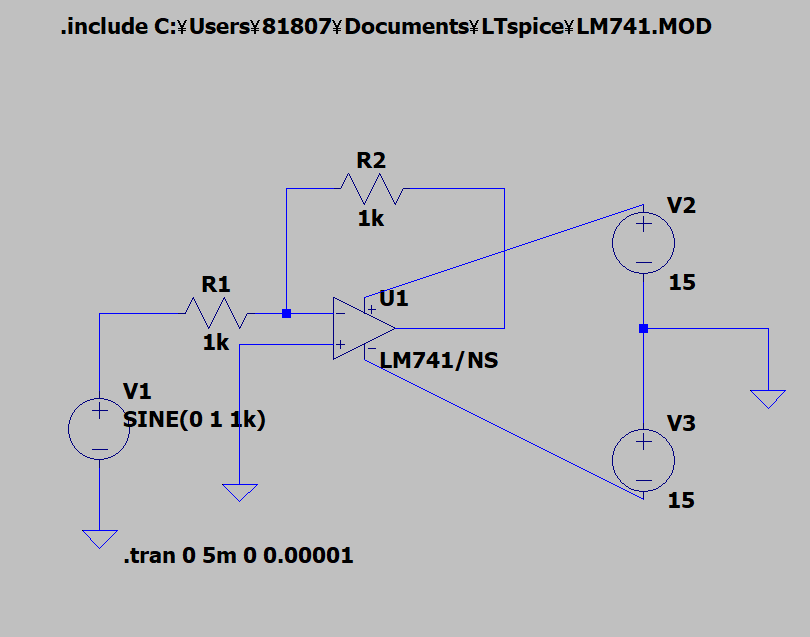
\includegraphics[scale=0.35]{kairozu5-31.png}
    \caption{$R_2 = 1\,\text{k}\Omega$}
\end{figure}
\begin{figure}[H]
    \centering
    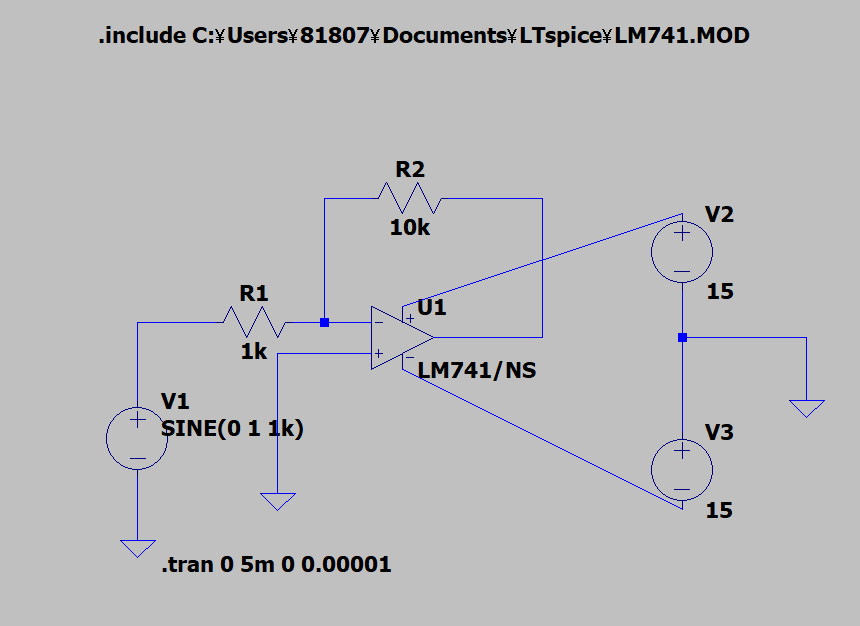
\includegraphics[scale=0.35]{kairozu5-32.png}
    \caption{$R_2 = 10\,\text{k}\Omega$}
\end{figure}
\begin{figure}[H]
    \centering
    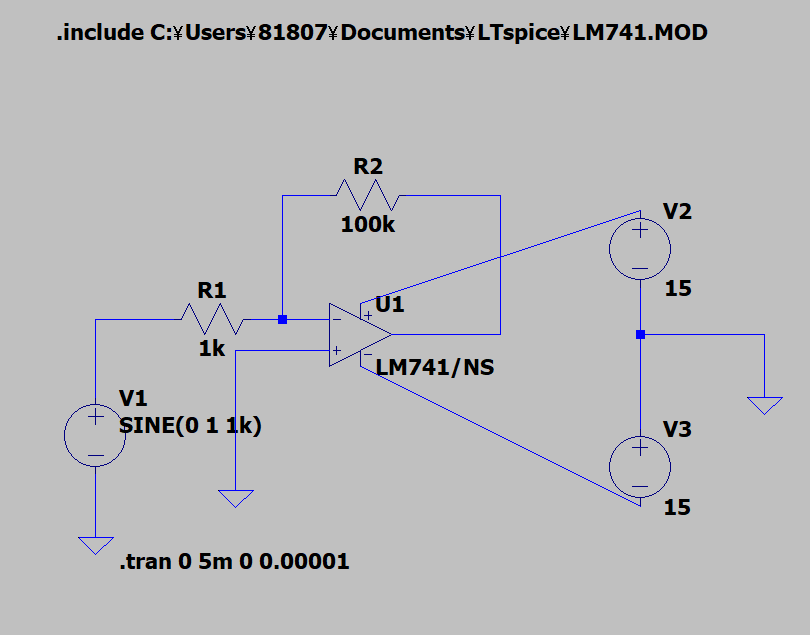
\includegraphics[scale=0.35]{kairozu5-33.png}
    \caption{$R_2 = 100\,\text{k}\Omega$}
\end{figure}

\item $R_1 = 1\,\text{k}\Omega $ に対し,$R_2 = 1\,\text{k}, 10\,\text{k}, 100\,\text{k}\Omega$と設定したときの周波数特性 (振幅特性と位相特性) を
観察した。
以下にLTspiceにより作成した回路図を示す。
\begin{figure}[H]
    \centering
    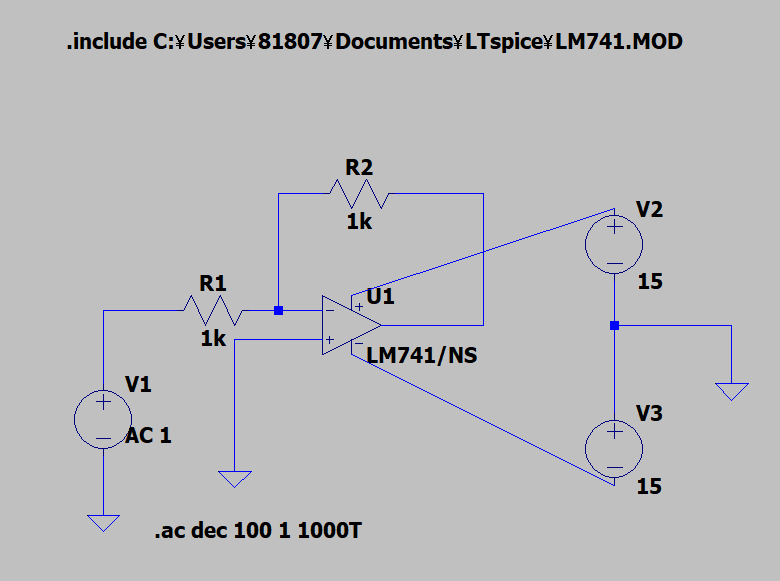
\includegraphics[scale=0.35]{kairozu5-41.png}
    \caption{$R_2 = 1\,\text{k}\Omega$}
\end{figure}
\begin{figure}[H]
    \centering
    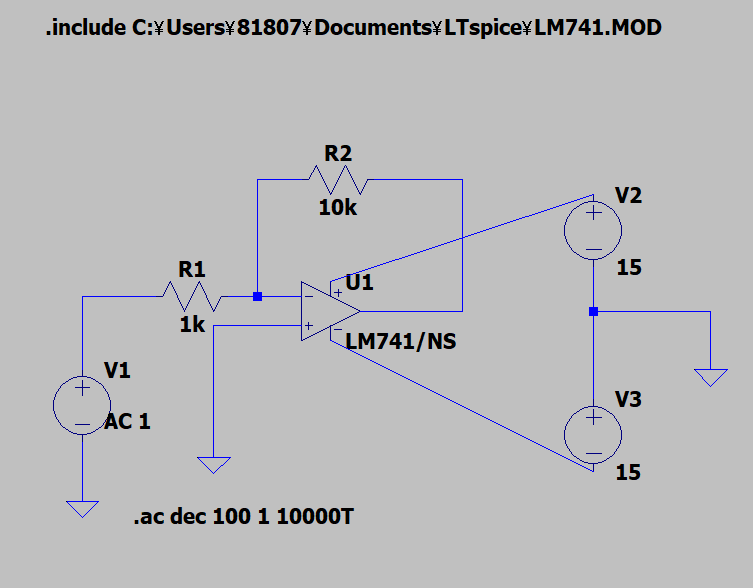
\includegraphics[scale=0.35]{kairozu5-42.png}
    \caption{$R_2 = 10\,\text{k}\Omega$}
\end{figure}
\begin{figure}[H]
    \centering
    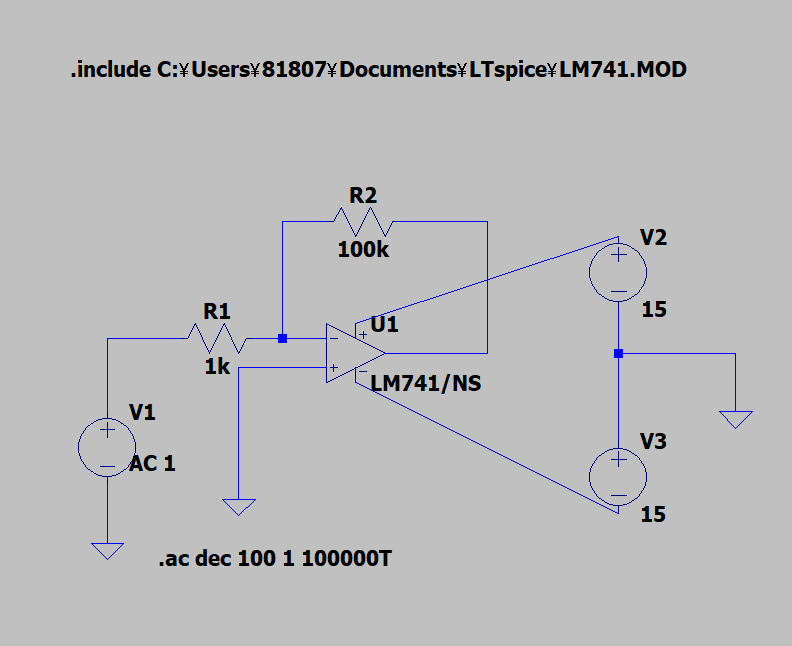
\includegraphics[scale=0.35]{kairozu5-43.png}
    \caption{$R_2 = 100\,\text{k}\Omega$}
\end{figure}
\end{enumerate}

\subsubsection{結果}
以下に各$R_2$に対する解析結果示す。
\begin{figure}[H]
    \centering
    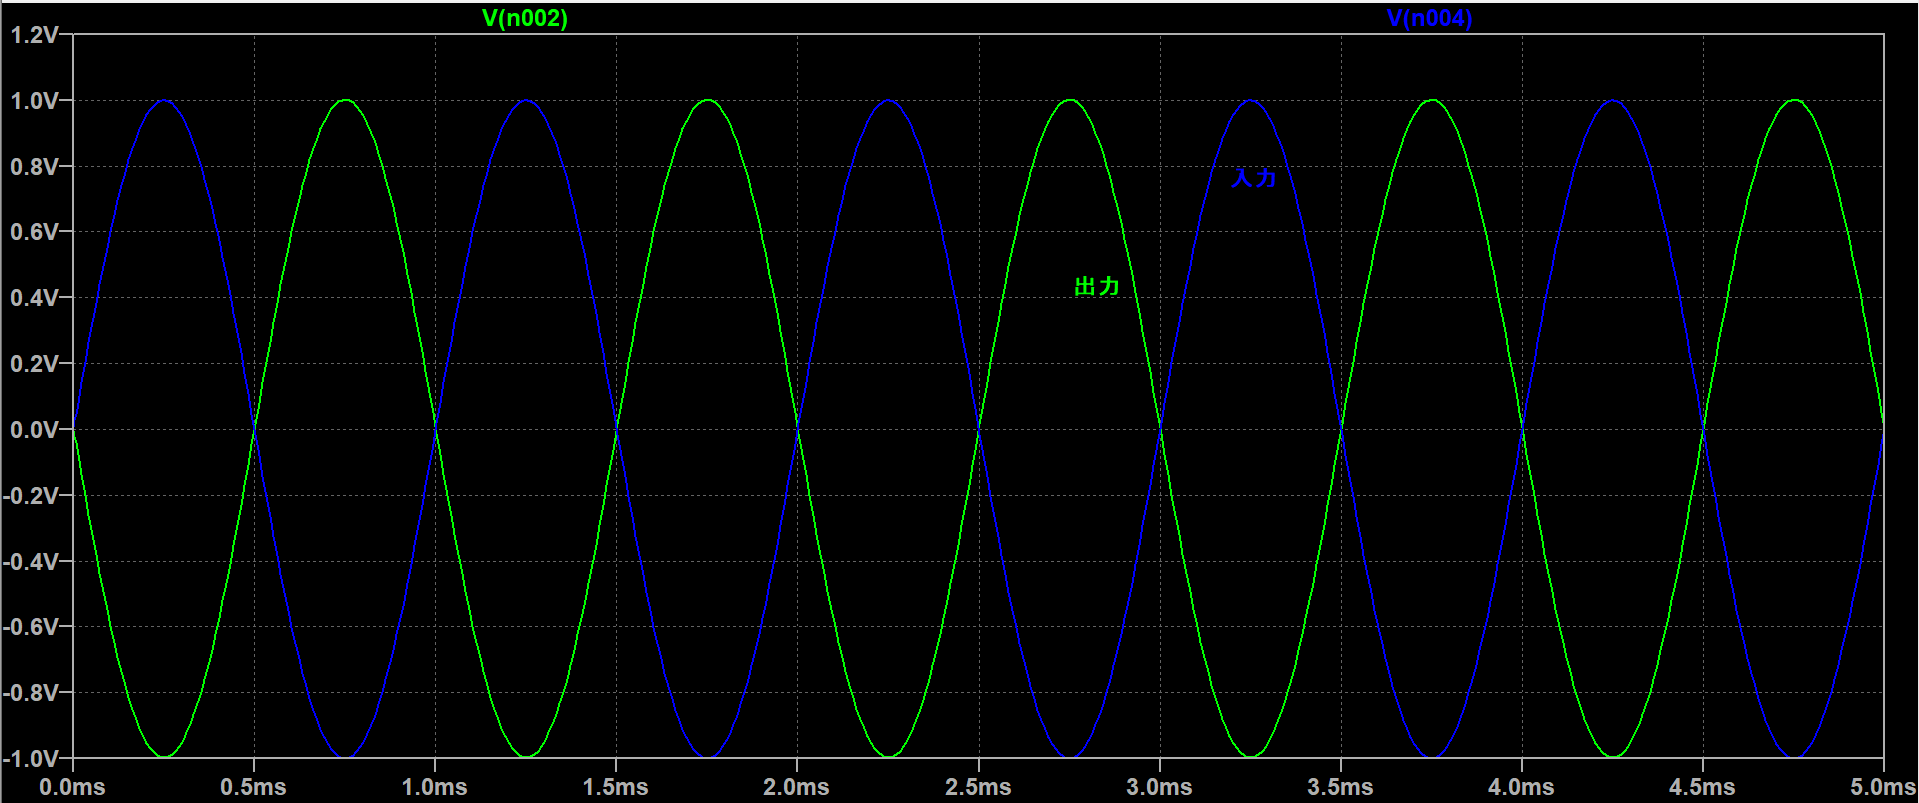
\includegraphics[scale=0.25]{sim5-31.png}
    \caption{$R_2 = 1\,\text{k}\Omega$}
\end{figure}
\begin{figure}[H]
    \centering
    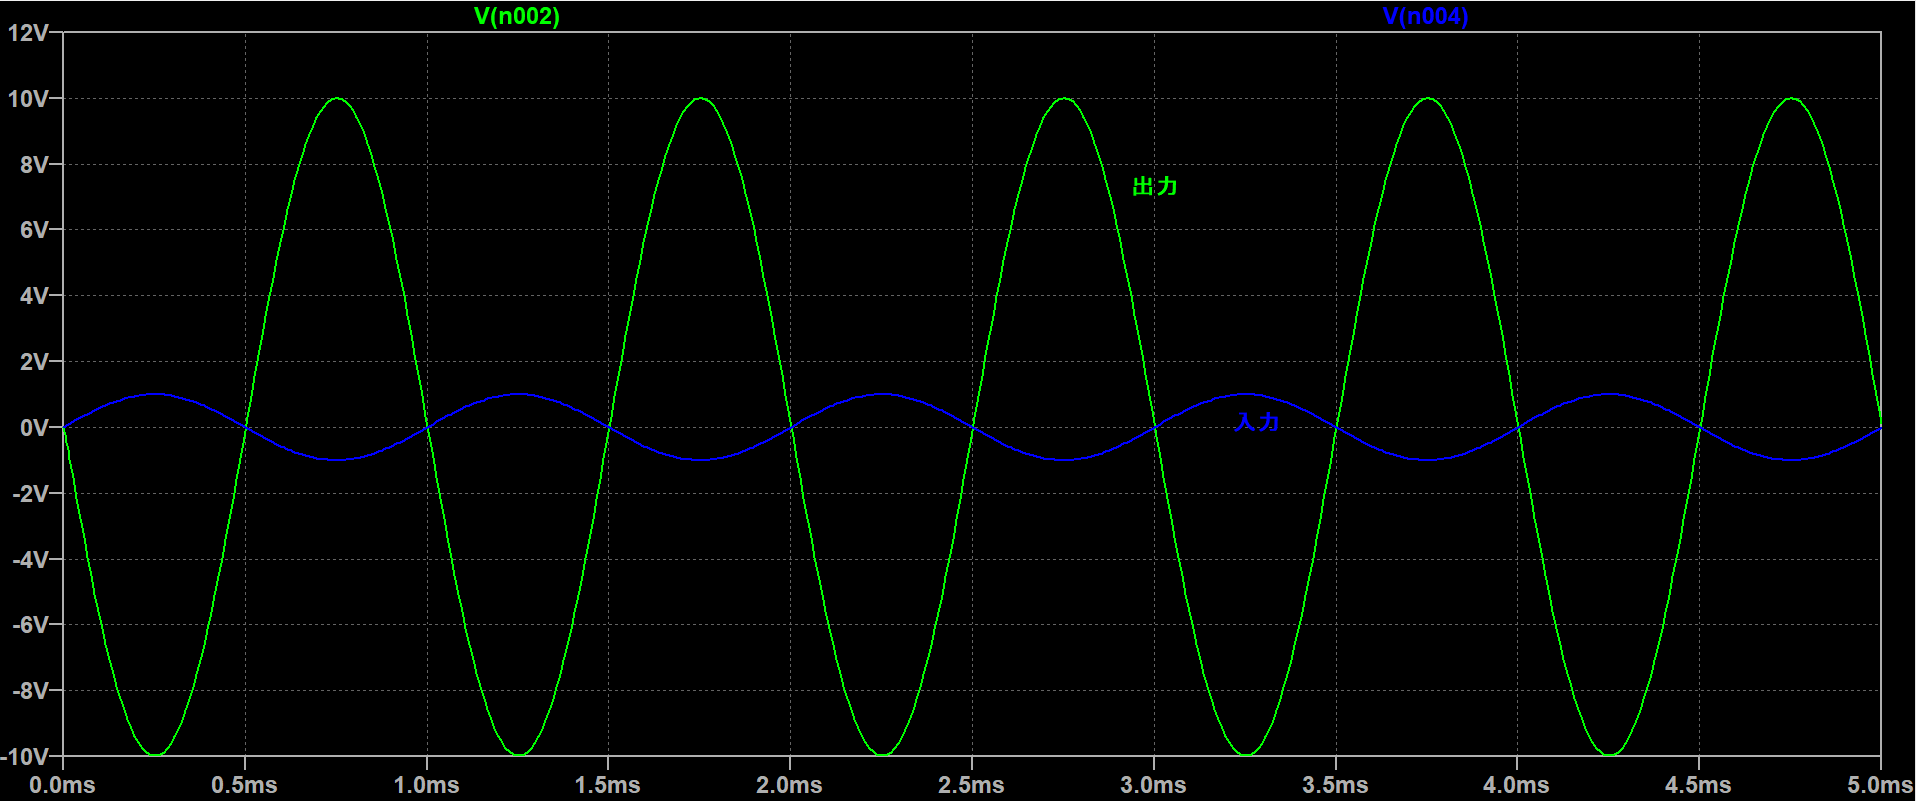
\includegraphics[scale=0.25]{sim5-32.png}
    \caption{$R_2 = 10\,\text{k}\Omega$}
\end{figure}
\begin{figure}[H]
    \centering
    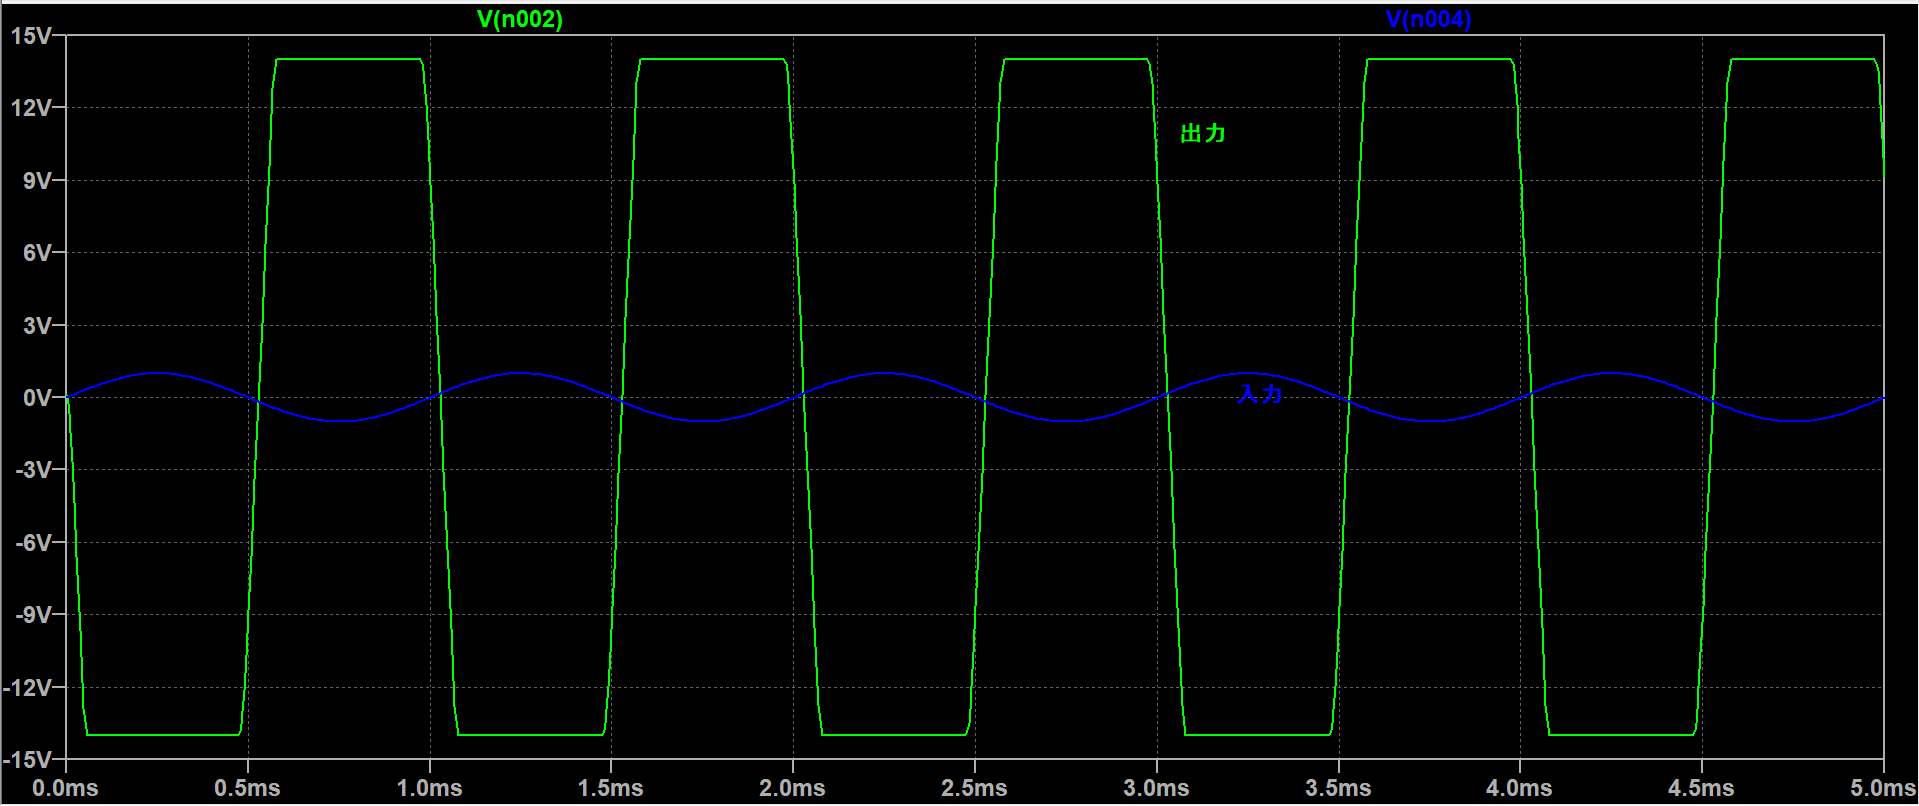
\includegraphics[scale=0.25]{sim5-33.png}
    \caption{$R_2 = 100\,\text{k}\Omega$}
\end{figure}

\begin{figure}[H]
    \centering
    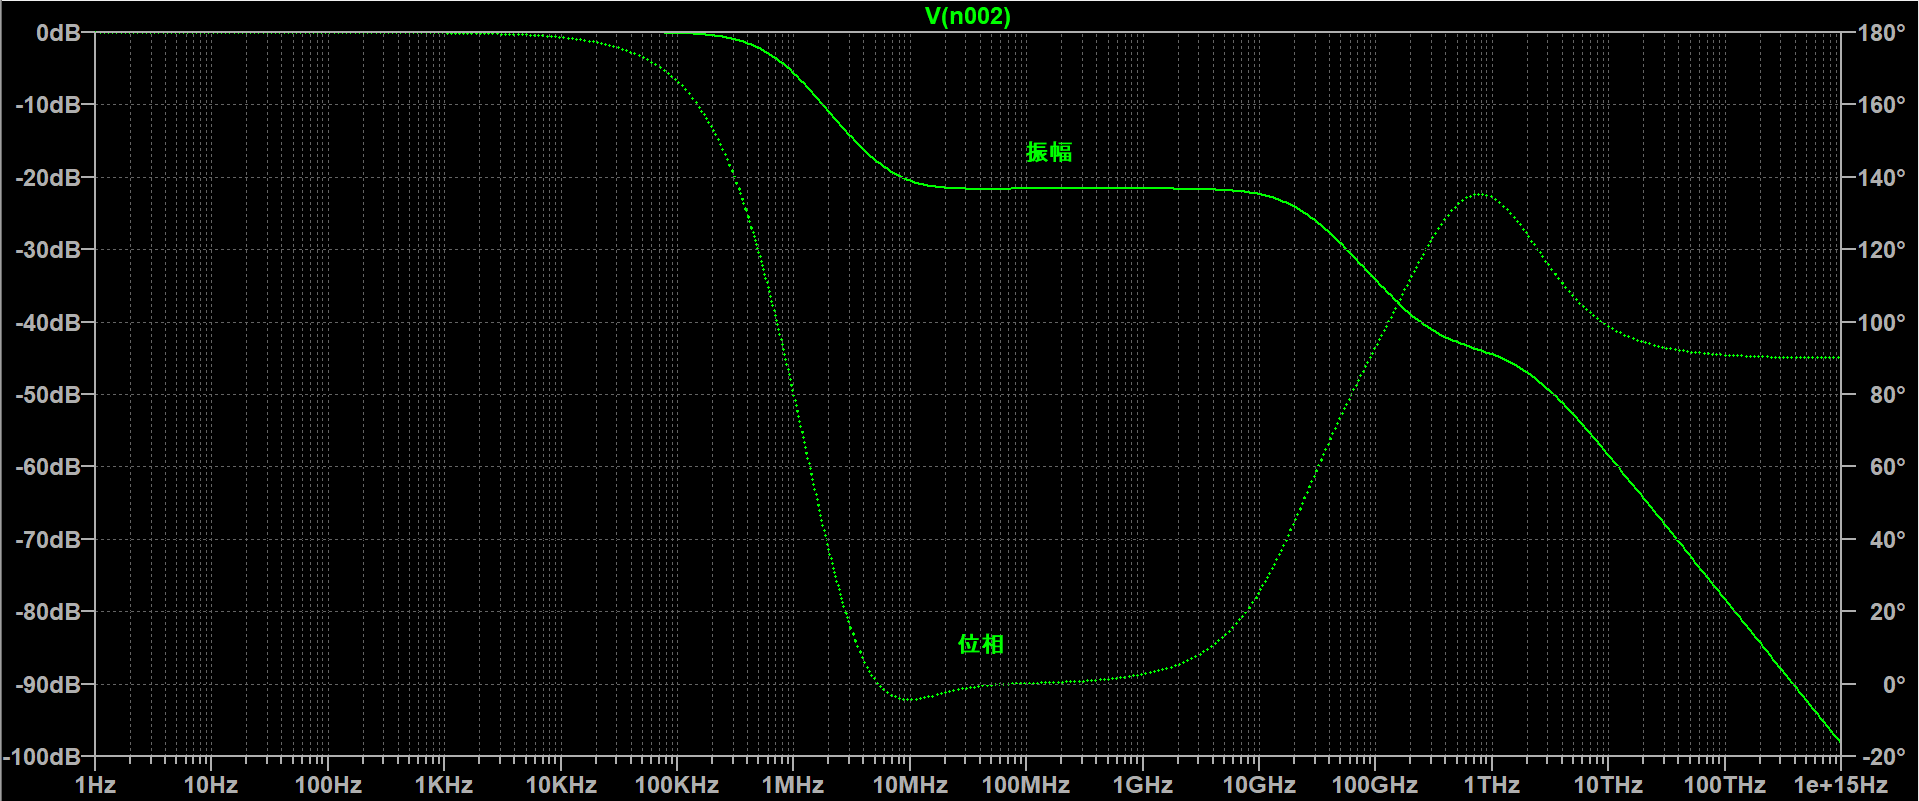
\includegraphics[scale=0.25]{sim5-41.png}
    \caption{$R_2 = 1\,\text{k}\Omega$}
\end{figure}
\begin{figure}[H]
    \centering
    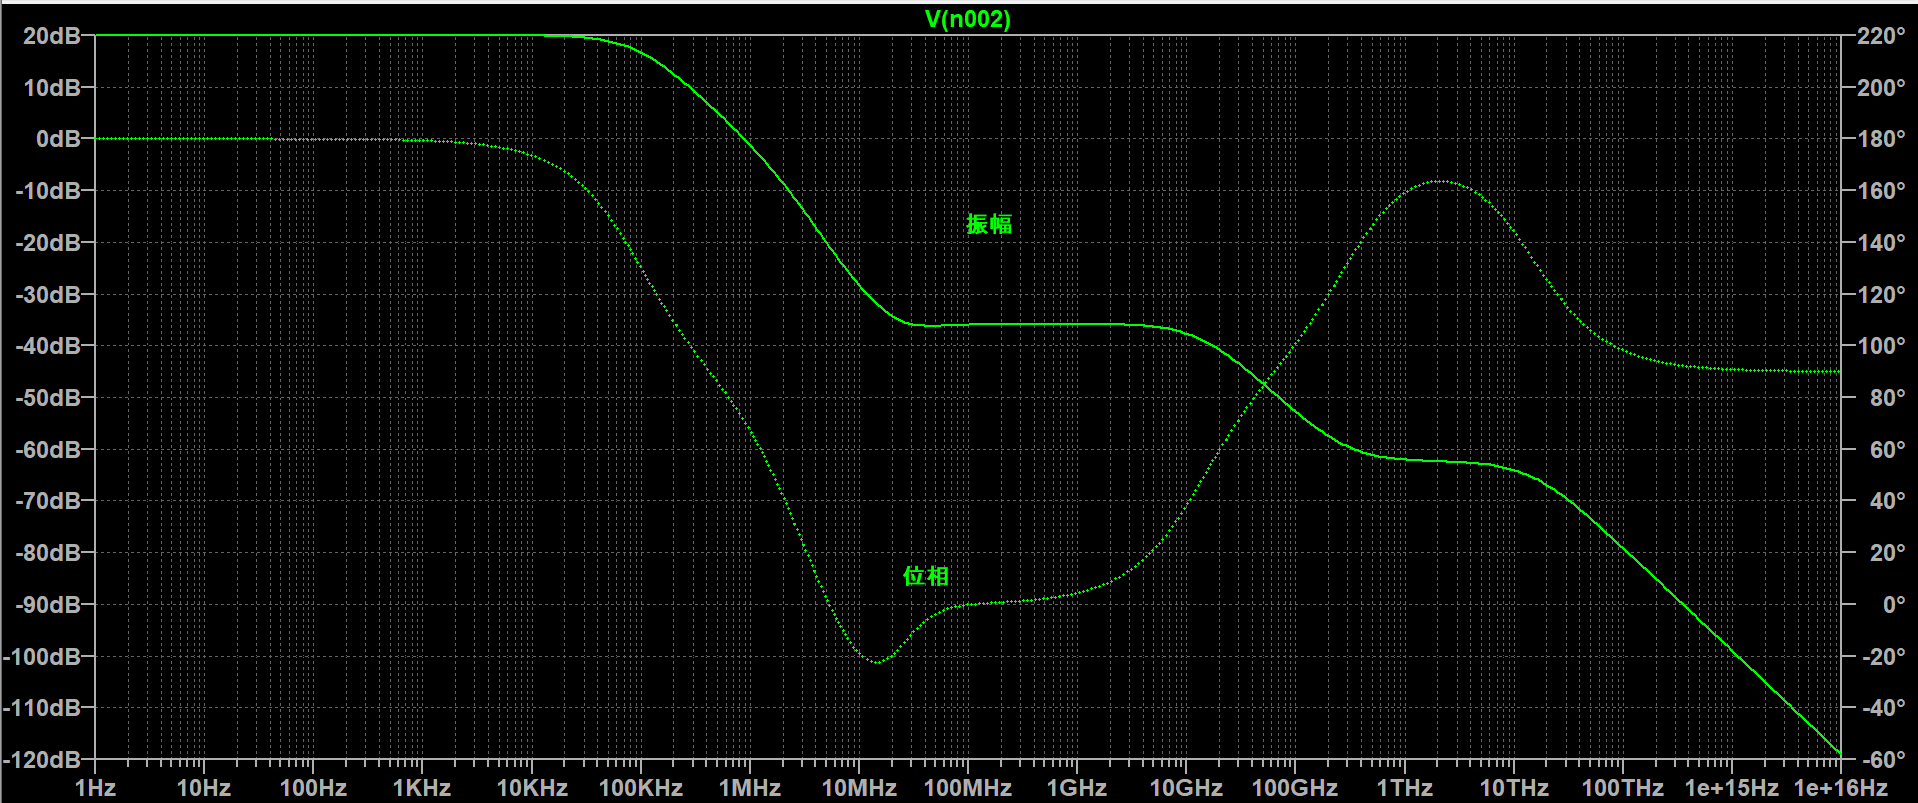
\includegraphics[scale=0.25]{sim5-42.png}
    \caption{$R_2 = 10\,\text{k}\Omega$}
\end{figure}
\begin{figure}[H]
    \centering
    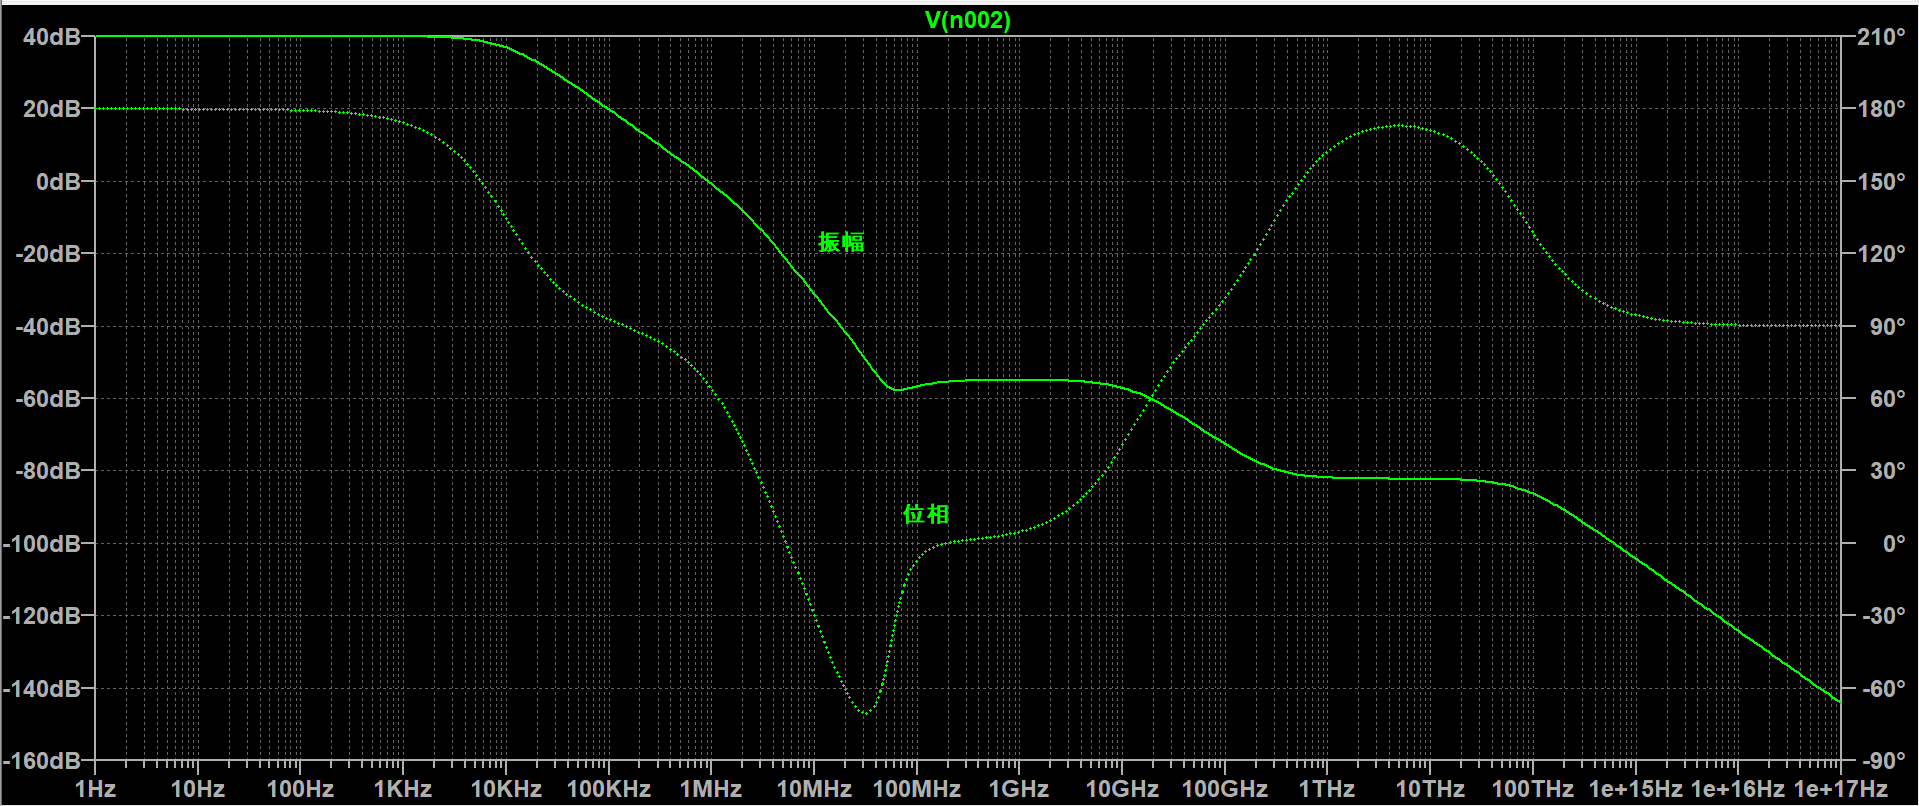
\includegraphics[scale=0.25]{sim5-43.png}
    \caption{$R_2 = 100\,\text{k}\Omega$}
\end{figure}
\subsubsection{考察}
\paragraph{考察1}\mbox{}\\
反転増幅回路では、理想的な増幅率は
\[
A_v=-\frac{R_2}{R_1}
\]
で表される。今回、$R_1=1\,\mathrm{k\Omega}$ としたため、$R_2=1\,\mathrm{k\Omega}$、$10\,\mathrm{k\Omega}$、$100\,\mathrm{k\Omega}$ の場合の理論上の増幅率はそれぞれ
\[
A_v=-1,\quad -10,\quad -100
\]
となる。したがって、出力波形は入力波形に対して反転し、$R_2$ を大きくするほど出力振幅も大きくなる。

実際の時間波形でも、$R_2=1\,\mathrm{k\Omega}$ の場合には入力とほぼ同じ大きさの反転波形が得られ、$R_2=10\,\mathrm{k\Omega}$ の場合には出力振幅がおよそ10倍となった。一方、$R_2=100\,\mathrm{k\Omega}$ の場合には理論上は100倍の増幅となるが、出力電圧が電源電圧による制限を超えるため、波形が大きく歪み、クリップが発生した。したがって、$R_2$ を大きくすれば増幅率は大きくなるが、出力可能な電圧範囲を超えると正常な正弦波として出力できなくなることが分かる。\\


周波数特性についても、$R_2$ を大きくするほど低周波側での振幅特性は大きくなった。これは、増幅率が $R_2/R_1$ に比例するためである。しかし、増幅率を大きくした場合には、高周波側で振幅特性が低下し始める周波数が低くなることが確認できる。つまり、大きな増幅率を得ようとすると、高い周波数まで同じ増幅率を保つことが難しくなる。このことから、反転増幅回路では、増幅率と使用できる周波数範囲の間に関係があることが分かる。

\paragraph{考察2}\mbox{}\\
内部インピーダンスが $600\,\Omega$ のマイクロホンを入力に接続する場合を考える。反転増幅回路では、入力インピーダンスはおおよそ $R_1$ で決まる。そのため、$R_1$ が $600\,\Omega$ に近すぎると、マイクロホン側に負荷がかかり、入力信号が十分に回路へ伝わらない可能性がある。したがって、$R_1$ は少なくとも $600\,\Omega$ より十分大きくする必要がある。

一方で、$R_2=10\,\mathrm{k\Omega}$ に固定した場合、増幅率は
\[
A_v=-\frac{10\,\mathrm{k\Omega}}{R_1}
\]
となるため、$R_1$ を大きくしすぎると増幅率が小さくなる。マイクロホンの信号は一般に小さいため、ある程度の増幅率も必要である。したがって、入力インピーダンスを確保しつつ、増幅率も小さくなりすぎないようにするには、$R_1$ は数 $\mathrm{k\Omega}$ 程度、例えば
\[
3\,\mathrm{k\Omega} \sim 10\,\mathrm{k\Omega}
\]
程度に設定するのが適切であると考えられる。



\section{実験2}
以下に実験2で用いた回路を示す。

\begin{figure}[H]
    \centering

    \begin{minipage}{0.48\linewidth}
        \centering
        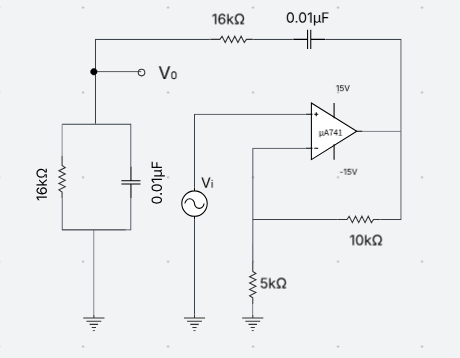
\includegraphics[width=\linewidth]{seikikann.png}
        \caption{正帰還回路}
    \end{minipage}
    \hfill
    \begin{minipage}{0.48\linewidth}
        \centering
        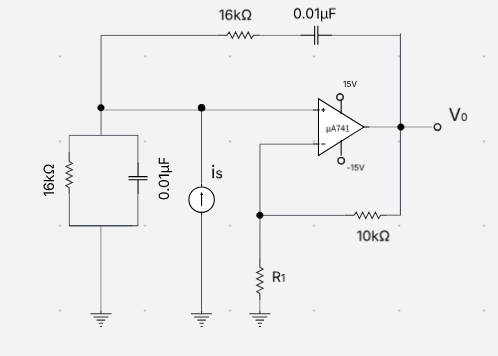
\includegraphics[width=\linewidth]{hassinn.png}
        \caption{発振回路}
    \end{minipage}

\end{figure}

\subsection{正帰還回路の応答}
\subsubsection{実験内容}


図27の回路において、入力電源 $V_i$ として振幅 $V_{\mathrm{AMPL}} = 1\,\mathrm{V}$ の正弦波を加え、
正弦波の周波数を $500\,\mathrm{Hz}$、$1\,\mathrm{kHz}$、$2\,\mathrm{kHz}$ としたときの出力応答 $V_o$ を観察した。
以下にLTspiceにより作成した回路図を示す。

\begin{figure}[H]
    \centering
    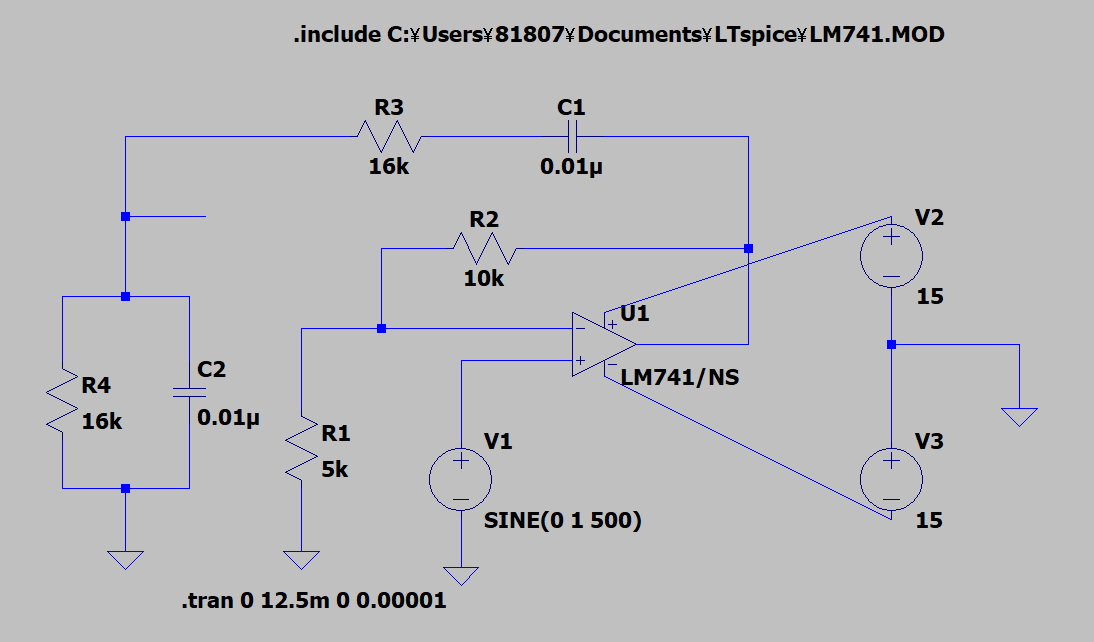
\includegraphics[scale=0.35]{kairozu5-51.png}
    \caption{$f = 500\,\text{Hz}$}
\end{figure}
\begin{figure}[H]
    \centering
    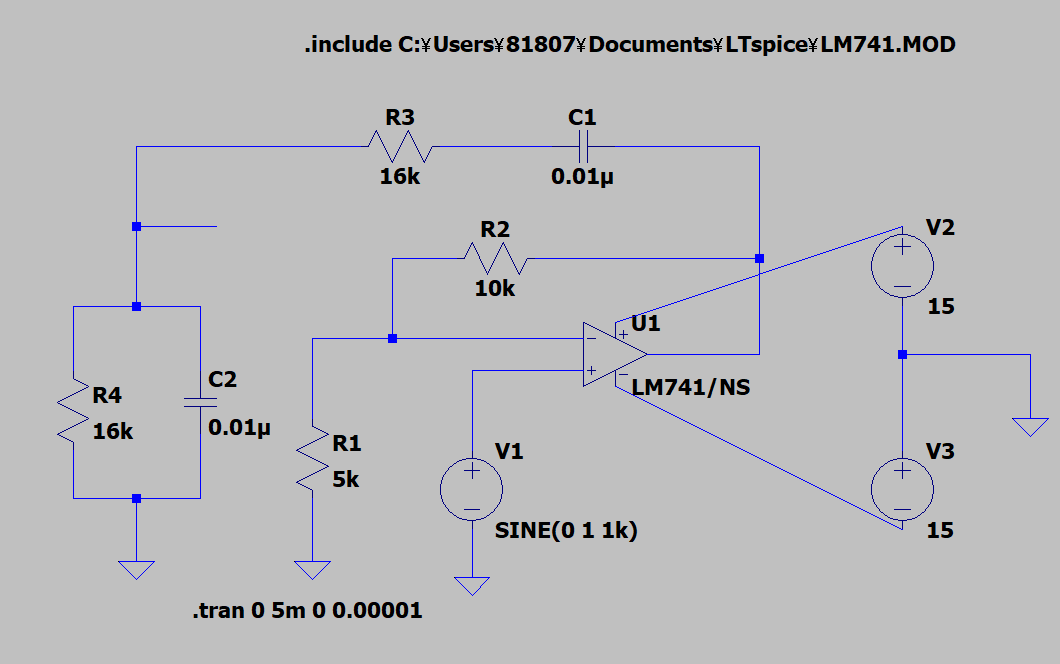
\includegraphics[scale=0.35]{kairozu5-52.png}
    \caption{$f = 1\,\text{kHz}$}
\end{figure}
\begin{figure}[H]
    \centering
    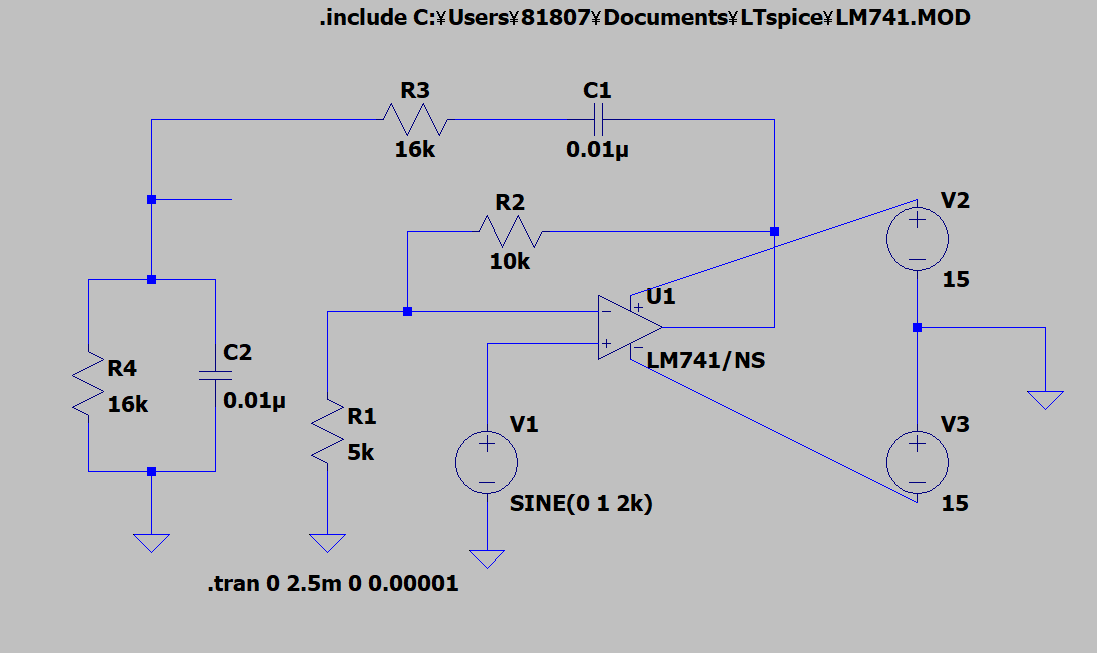
\includegraphics[scale=0.35]{kairozu5-53.png}
    \caption{$f = 2\,\text{kHz}$}
\end{figure}

\subsubsection{結果}
\begin{figure}[H]
    \centering
    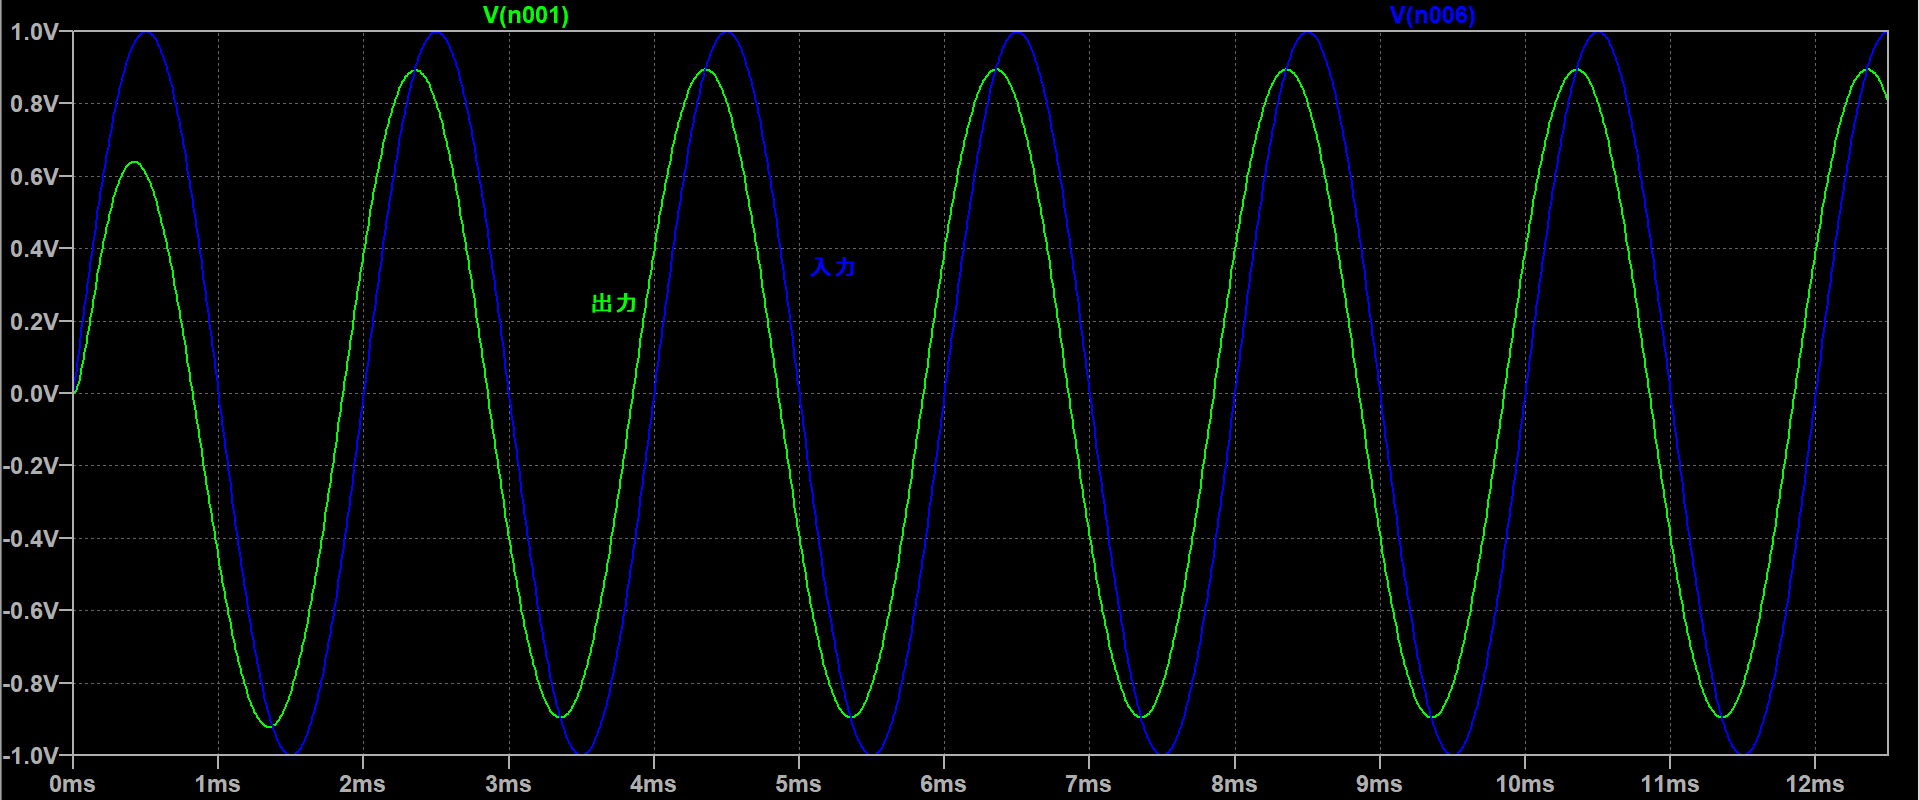
\includegraphics[scale=0.25]{sim5-51.png}
    \caption{$f = 500\,\text{Hz}$}
\end{figure}
\begin{figure}[H]
    \centering
    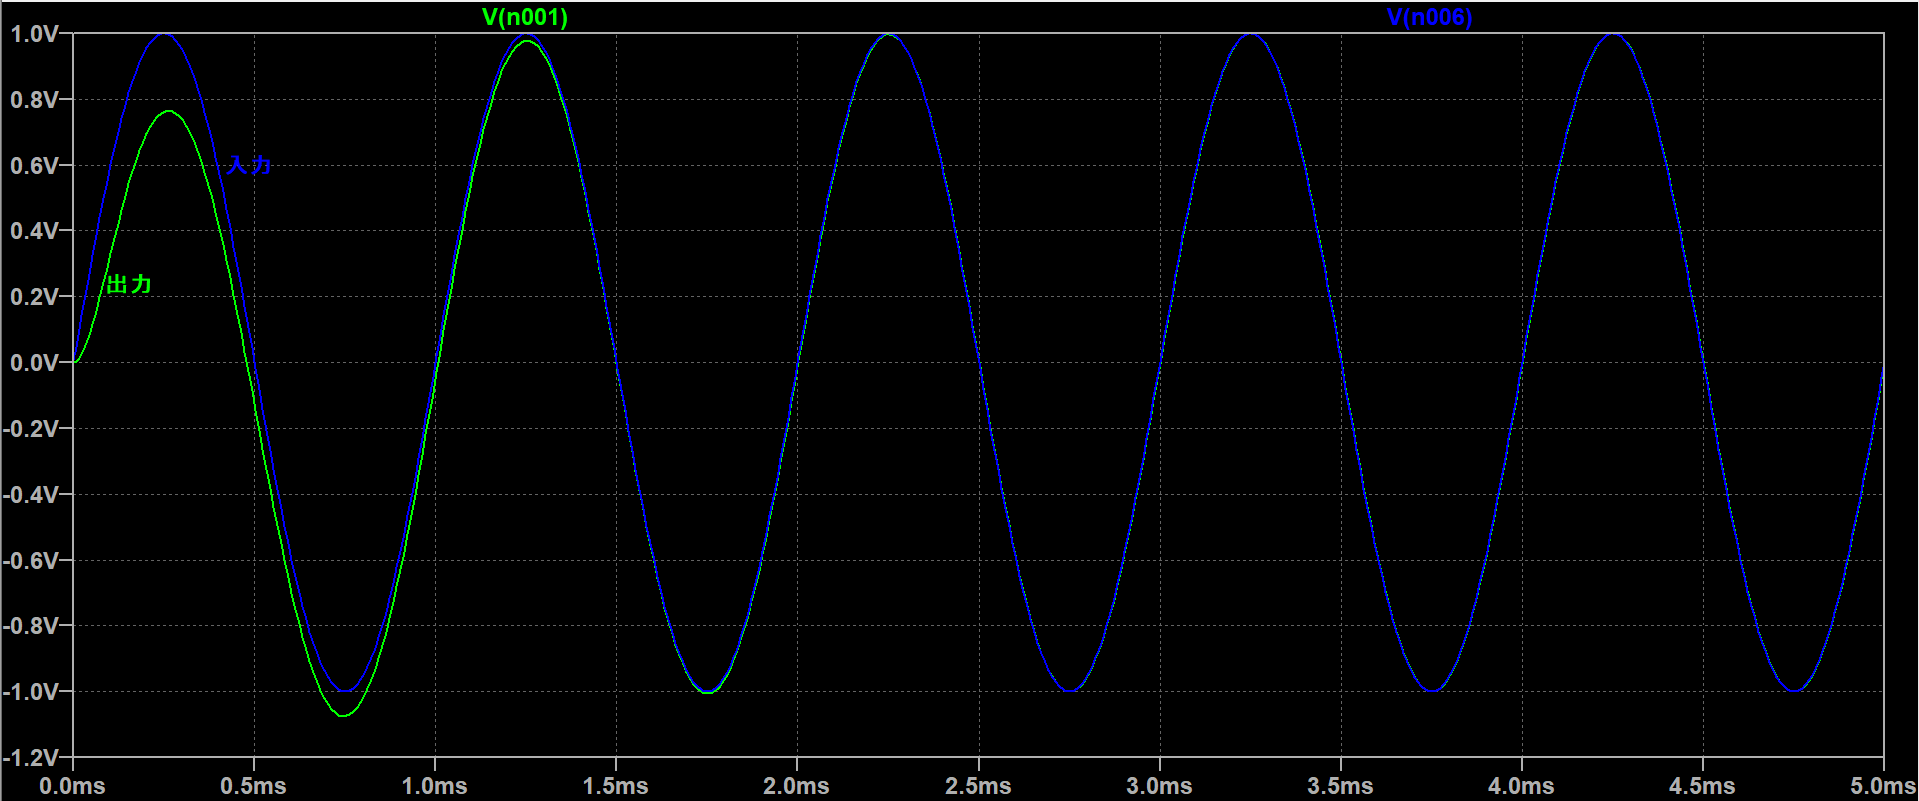
\includegraphics[scale=0.25]{sim5-52.png}
    \caption{$f = 1\,\text{kHz}$}
\end{figure}
\begin{figure}[H]
    \centering
    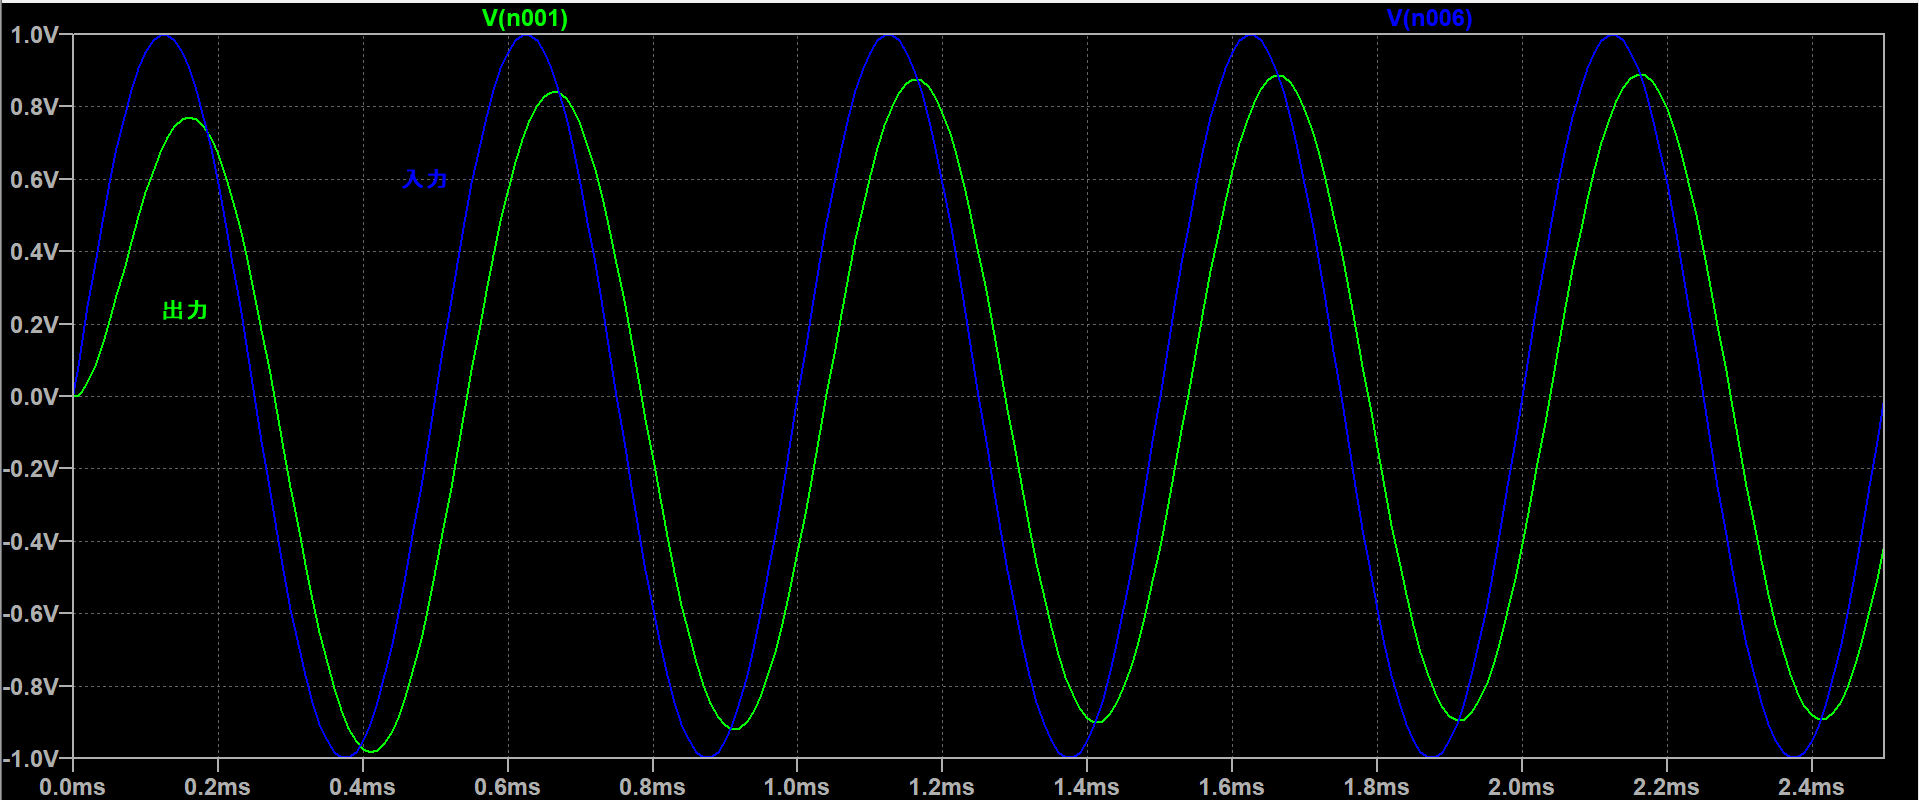
\includegraphics[scale=0.25]{sim5-53.png}
    \caption{$f = 2\,\text{kHz}$}
\end{figure}




\subsection{発振出力の観察}
\subsubsection{実験内容}
図28の回路について抵抗 $R_1$ を $4.95\,\mathrm{k\Omega}$、$5.00\,\mathrm{k\Omega}$、$5.05\,\mathrm{k\Omega}$ としたときの
出力波形 $V_O$ を観察した。
以下にLTspiceにより作成した回路図を示す。

\begin{figure}[H]
    \centering
    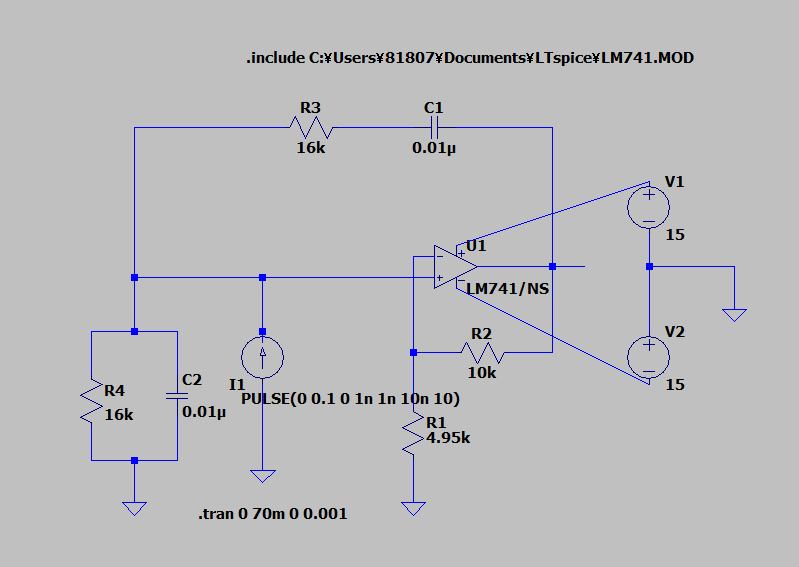
\includegraphics[scale=0.35]{kairozu5-61.png}
    \caption{$f = 500\,\text{Hz}$}
\end{figure}
\begin{figure}[H]
    \centering
    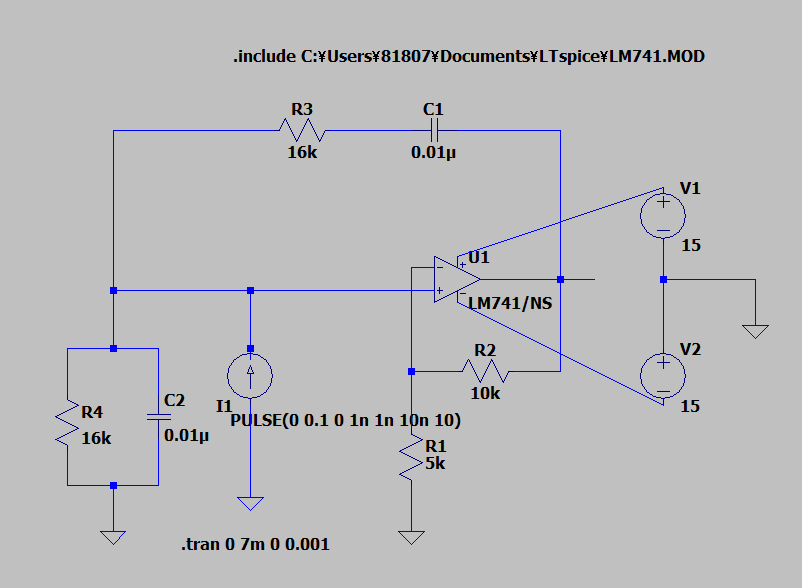
\includegraphics[scale=0.35]{kairozu5-62.png}
    \caption{$f = 1\,\text{kHz}$}
\end{figure}
\begin{figure}[H]
    \centering
    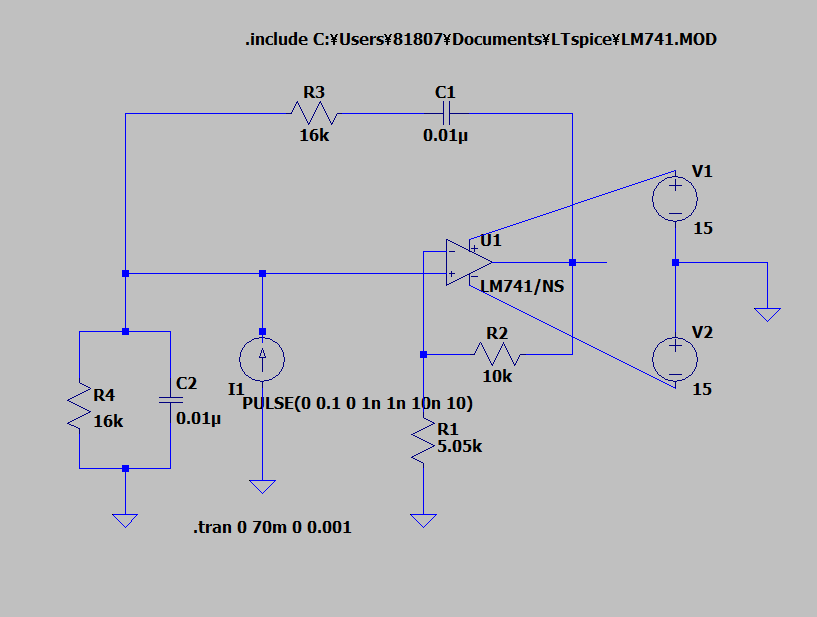
\includegraphics[scale=0.35]{kairozu5-63.png}
    \caption{$f = 2\,\text{kHz}$}
\end{figure}

\subsubsection{結果}

\begin{figure}[H]
    \centering
    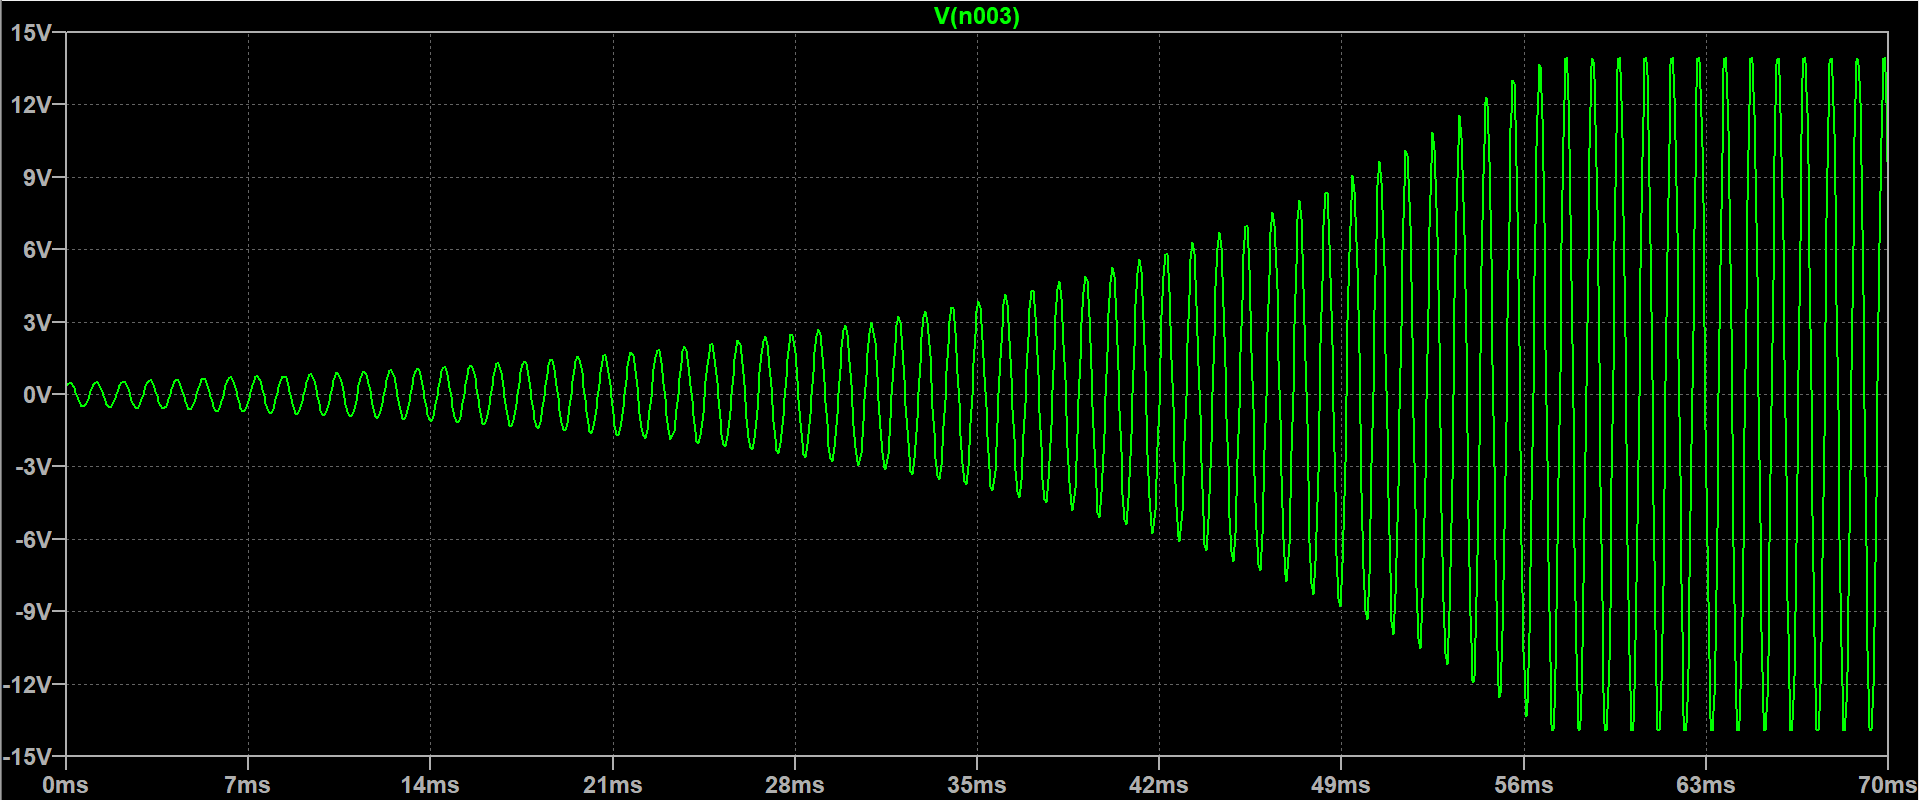
\includegraphics[scale=0.25]{sim5-61.png}
    \caption{$f = 500\,\text{Hz}$}
\end{figure}
\begin{figure}[H]
    \centering
    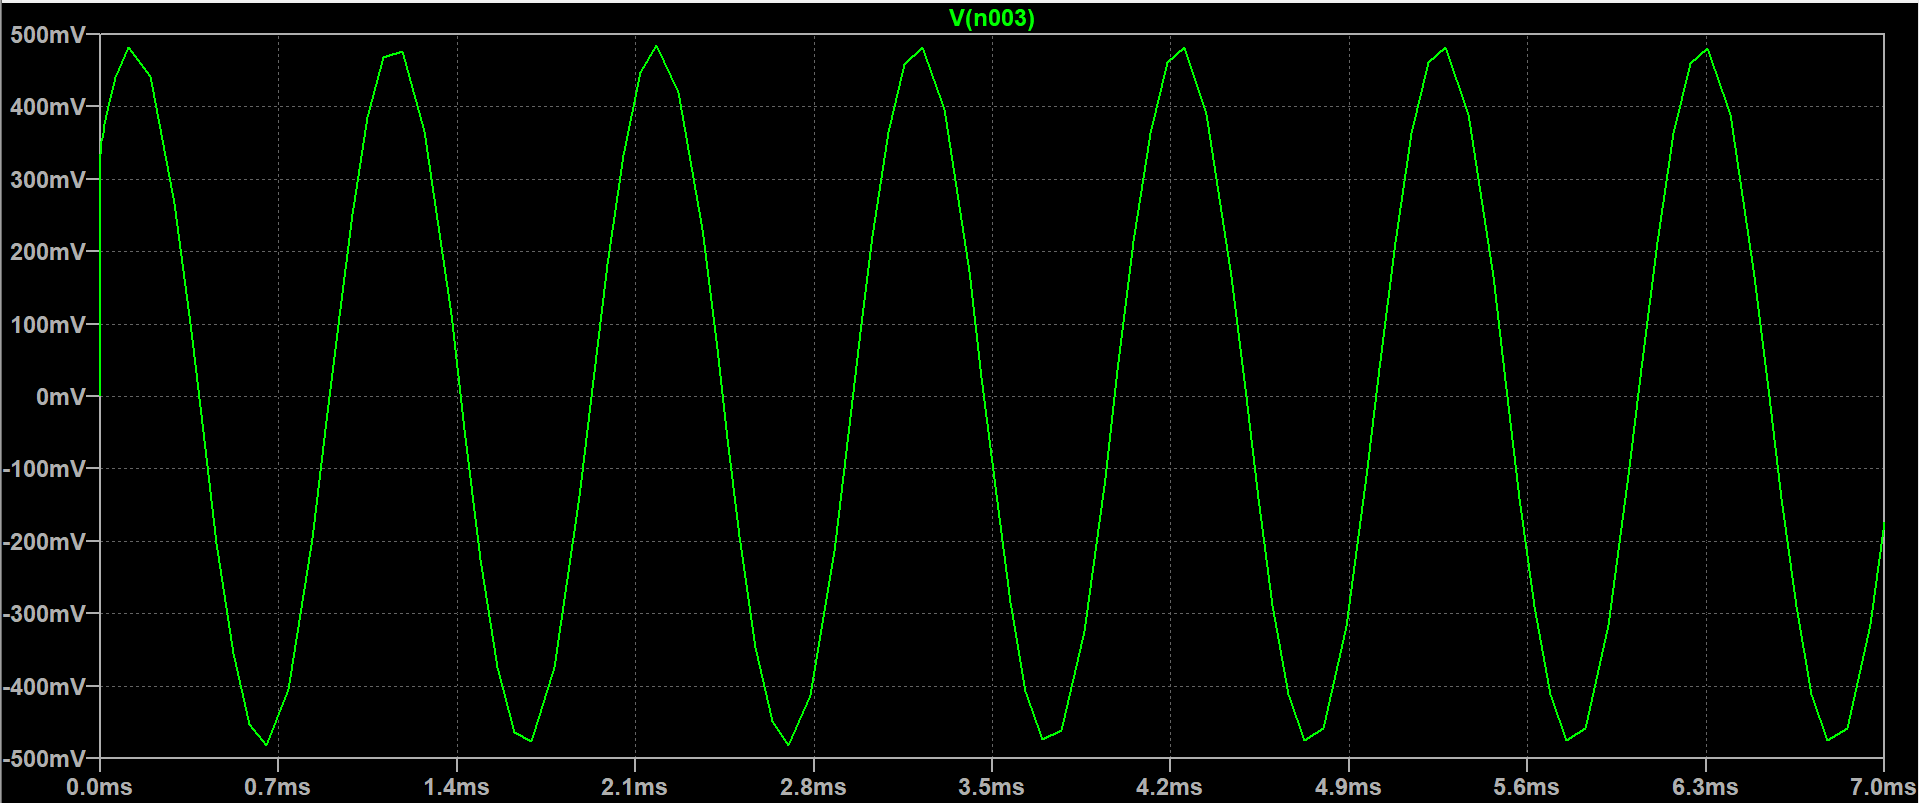
\includegraphics[scale=0.25]{sim5-62.png}
    \caption{$f = 1\,\text{kHz}$}
\end{figure}
\begin{figure}[H]
    \centering
    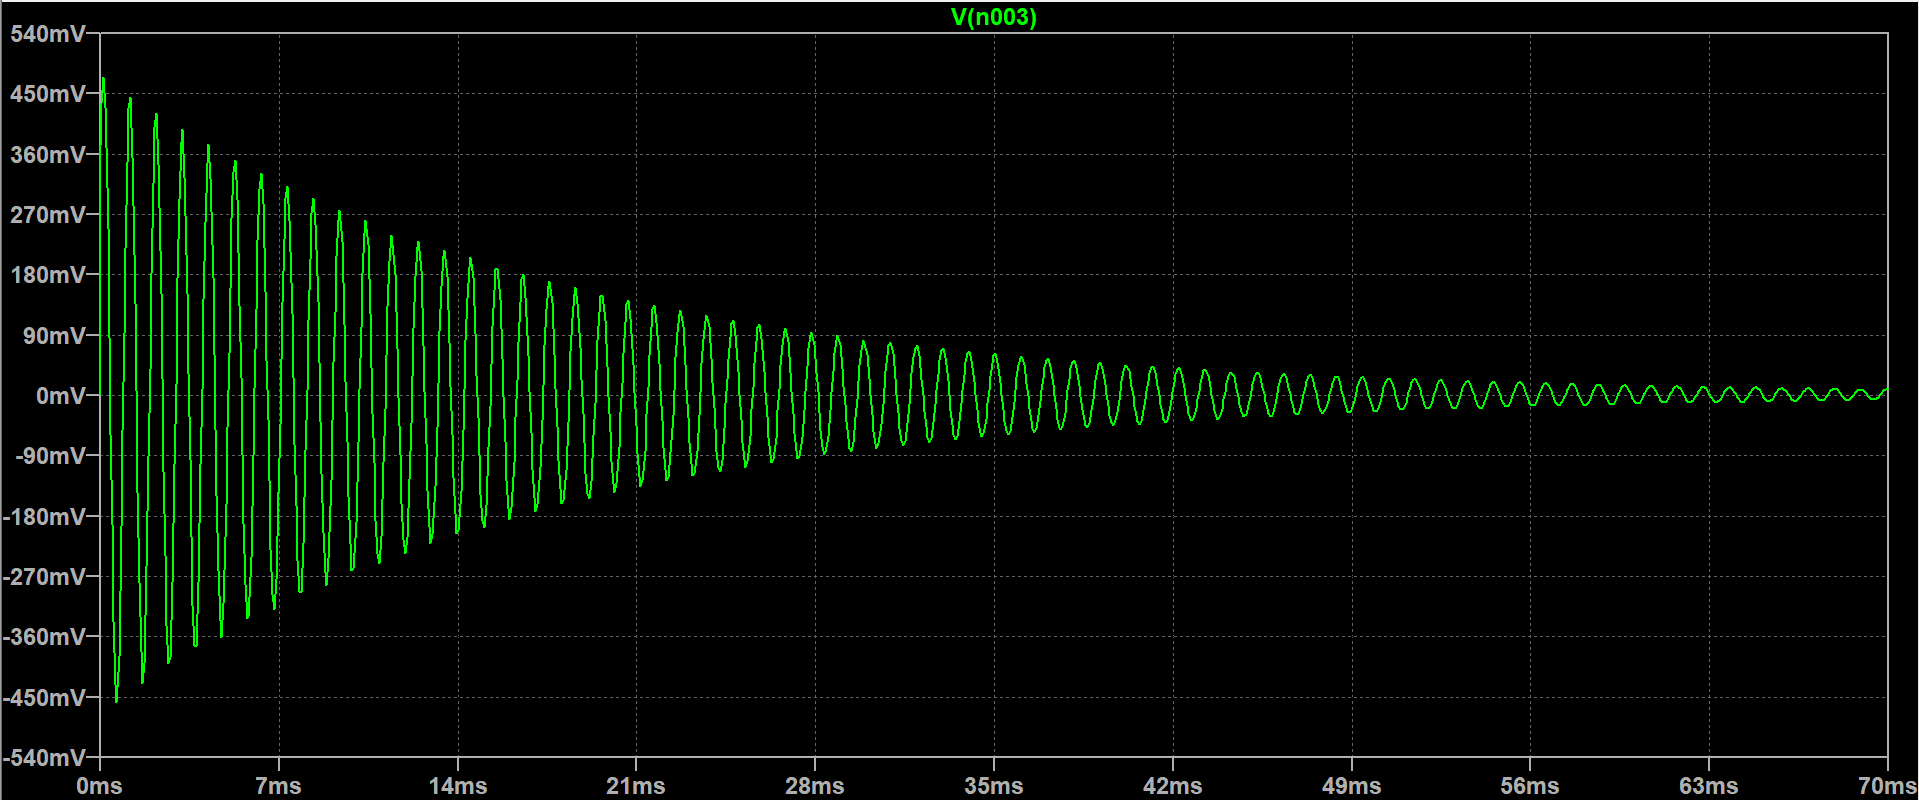
\includegraphics[scale=0.25]{sim5-63.png}
    \caption{$f = 2\,\text{kHz}$}
\end{figure}



\subsection{自由課題}

\subsubsection{実験内容}
帰還回路のコンデンサ $C$ を $0.01\,\mu\mathrm{F}$ に固定したとき、表2のルールで割り当てられた
周波数で発振するように帰還回路の抵抗値を調整し、発振時の波形を観察せよ。
以下にLTspiceにより作成した回路図を示す。
\begin{figure}[H]
    \centering
    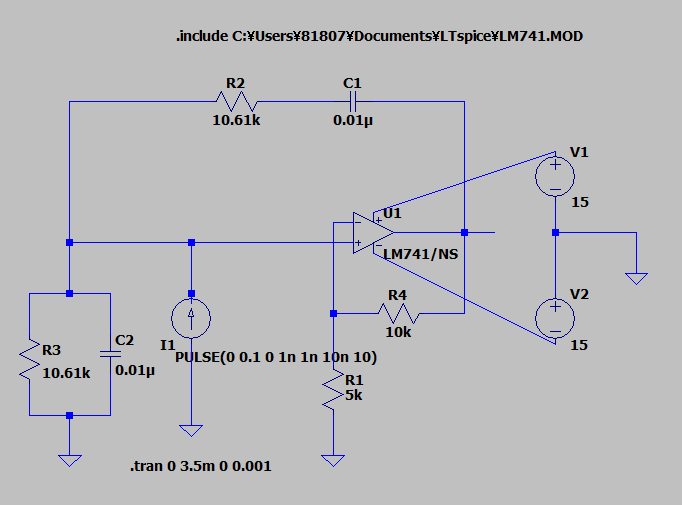
\includegraphics[scale=0.35]{kairozu5-7.png}
    \caption{$f = 1500\,\text{Hz}$}
\end{figure}
\subsubsection{結果}
\begin{figure}[H]
    \centering
    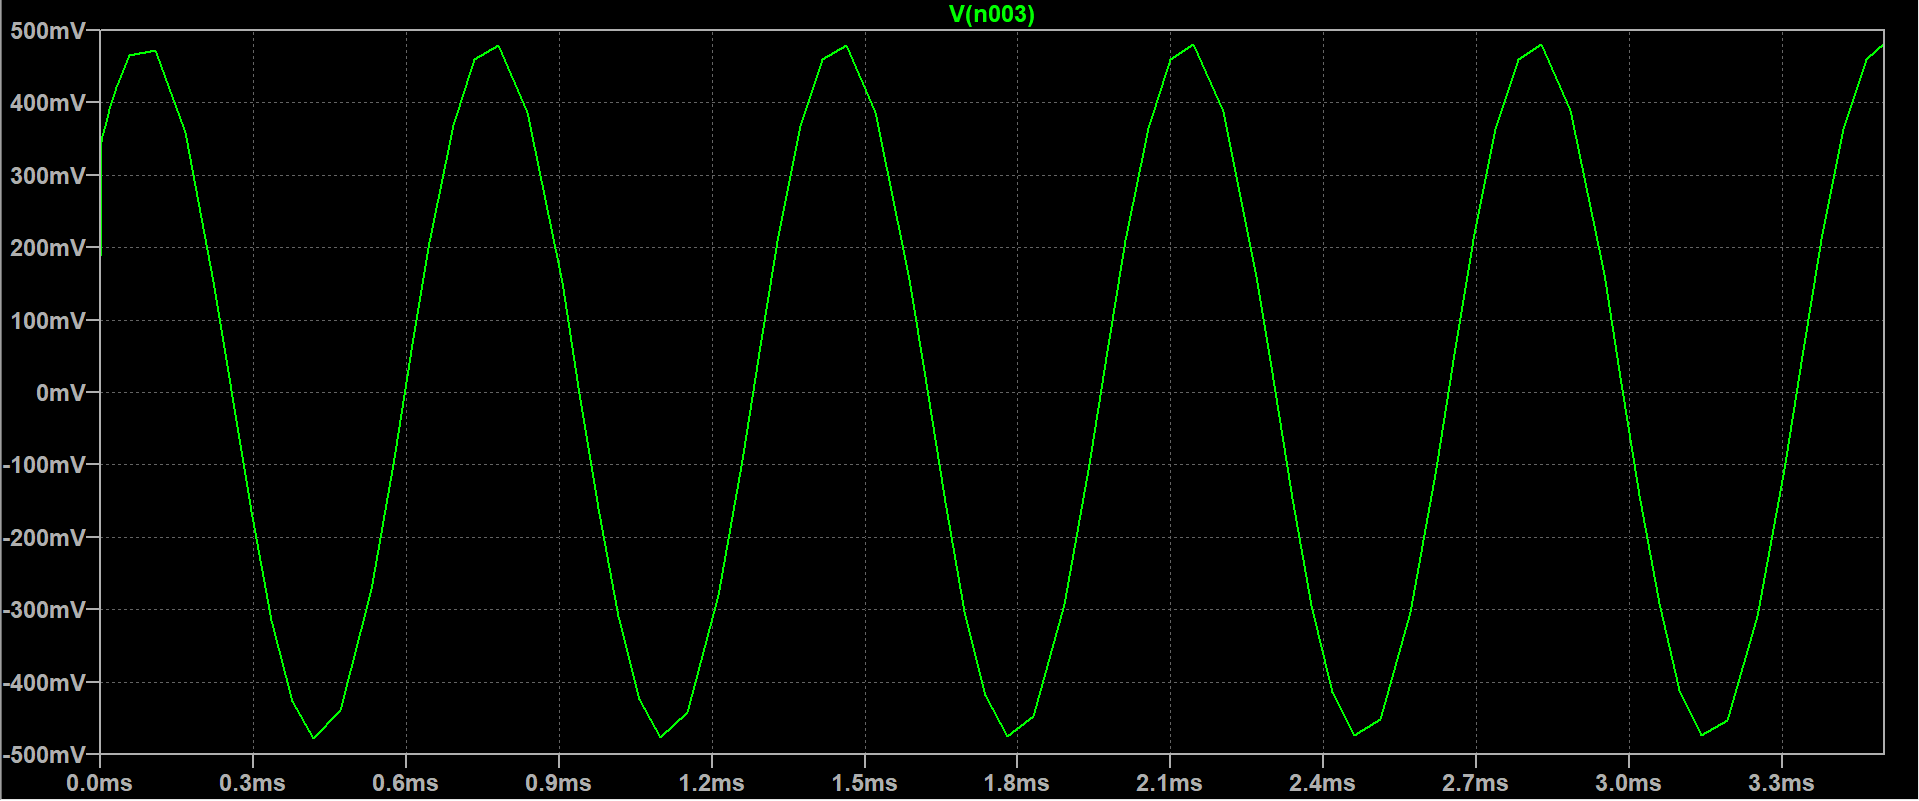
\includegraphics[scale=0.25]{sim5-7.png}
    \caption{$f = 2\,\text{kHz}$}
\end{figure}
\end{document}